% Asymmetric Society - bachelor thesis (ZAV-36)
% English body, Croatian front-matter labels (TVZ). IEEE numeric citations.
% Title page: TVZ naslovnica (Croatian), included as the first page (see \begin{titlepage} below).
% Build: tectonic (XeTeX). Native Croatian diacritics; biber bundled.
\documentclass[11pt,a4paper,oneside]{report}

% --- fonts (XeTeX via tectonic): fontspec defaults to bundled Latin Modern,
%     which has full Croatian glyph coverage and reads UTF-8 natively. ---
\usepackage{fontspec}
\usepackage[a4paper,margin=2.5cm]{geometry}
\linespread{1.13}

% --- graphics / tables / code ---
\usepackage{graphicx}
\graphicspath{{../figures/}}
\usepackage{booktabs}
\usepackage{multirow}
\usepackage{placeins}  % \FloatBarrier: keep each section's floats within it
\usepackage{xcolor}
\usepackage{listings}
\usepackage{caption}
\captionsetup{font=small,labelfont=bf}

% --- bibliography: classic bibtex + IEEEtran.bst (IEEE numeric). Robust in tectonic
%     (bundled bibtex, no biber/version coupling); same IEEE numeric result. ---

% --- links last ---
\usepackage[hidelinks]{hyperref}

% --- Furniture labels: English throughout (class defaults), except References and the
%     mandatory Croatian Sažetak page. The TVZ template has the final word at submission. ---
\renewcommand{\bibname}{References}
\renewcommand{\lstlistlistingname}{List of Listings}

% --- code listing style (self-contained; no shell-escape) ---
\definecolor{codebg}{HTML}{F4F2EE}
\definecolor{codekw}{HTML}{0072B2}
\definecolor{codecmt}{HTML}{6B6862}
\definecolor{codestr}{HTML}{009E73}
\lstdefinestyle{thesis}{
  basicstyle=\ttfamily\small,
  backgroundcolor=\color{codebg},
  keywordstyle=\color{codekw}\bfseries,
  commentstyle=\color{codecmt}\itshape,
  stringstyle=\color{codestr},
  numberstyle=\tiny\color{codecmt}, numbers=left, numbersep=8pt,
  breaklines=true, frame=single, rulecolor=\color{codecmt},
  showstringspaces=false, captionpos=b, language=Python, tabsize=4,
}
\lstset{style=thesis}
\AtBeginDocument{\counterwithin{lstlisting}{chapter}} % number listings per chapter (Listing 4.1), matching tables

% source line for captions (Autor for ours, [n] for borrowed)
\newcommand{\source}[1]{\par\smallskip{\footnotesize\textit{Source: #1}\par}}

\begin{document}

% ================= NASLOVNICA (TVZ) =================
\begin{titlepage}
    \centering

    % --- Zaglavlje: ustanova i studij ---
    {\large Tehničko veleučilište u Zagrebu\par}
    \vspace{0.4em}
    {\large Stručni prijediplomski studij Računarstvo\par}

    \vfill

    % --- Naslov rada: engleski (jezik rada) primarno, hrvatski prijevod ispod ---
    {\LARGE\bfseries Asymmetric Society: Capability Heterogeneity\\[0.3em]
    Among LLM Agents in Iterated Economic Games\par}

    \vspace{0.8em}

    {\large\itshape Asimetrično društvo: heterogenost sposobnosti\\[0.2em]
    među LLM agentima u iteriranim ekonomskim igrama\par}

    \vspace{1.0em}

    % --- Podnaslov ---
    {\large Završni rad\par}

    \vfill

    % --- Mentor i student (poravnato desno) ---
    \begin{flushright}
        \large
        \textbf{Ime i prezime mentora:}\\
        dr.\ sc.\ Aleksandar Stojanović\\[1.2em]
        \textbf{Ime i prezime studenta:}\\
        Francesco Marko Livaić\\
    \end{flushright}

    \vfill

    % --- Mjesto i datum ---
    {\large Zagreb, lipanj 2026.\par}

\end{titlepage}

% ================= FRONT MATTER =================
\pagenumbering{roman}

\chapter*{Sažetak}

Veliki jezični modeli različite sposobnosti sve se češće postavljaju zajedno, uz pretpostavku da
je jači agent u prednosti. Ova teza tu pretpostavku ispituje stavljajući tri jaka modela
(Claude Haiku~4.5, GPT-5-mini, Gemini~2.5 Flash) i jedan slab lokalni model (Llama~3.2 3B) u
ponovljene ekonomske igre, četveroigračku igru javnog dobra i dvoigračku igru povjerenja, kroz
matricu od šesnaest ćelija različitih sastava populacije, mjereći nejednakost, iskorištavanje i
obmanu kroz 320 unaprijed registriranih igara. Glavni nalaz obrće pretpostavku. Bez komunikacije
jaki modeli ostvaruju premiju sposobnosti; s komunikacijom se premija invertira i jaki modeli
zarađuju manje, a taj pomak model miješanih efekata smješta u grupnu igru i pokazuju ga sva tri
jaka modela pojedinačno. Poluga nije razmjena poruka: u ovom dizajnu poruka se bilježi, ali se
nikada ne dostavlja, pa je uvjet javno obavezivanje bez recepcije, a ponašanje mijenja okvir
traženja da se agent javno obveže, a ne išta što bi drugi agent pročitao. Učinak pripada grupnoj
igri i nestaje u dvoigračkoj razmjeni. Drugi, metodološki doprinos tiče se obmane: globalna
divergencija između izrečene i otkrivene politike agenta ocjenjuje najdosljednije suradnike kao
najmanje poštene, što je artefakt koncentracije ponašanja, dok istodobna mjera iznenađenja
(\textit{surprisal}) po potezu ispravno razdvaja razine. Fiksirani u smjeru prije nego što su
podaci postojali, rezultati upozoravaju da sposobnost ne mora donijeti prednost, da traženje od
agenata da se obvežu može staviti sposobne u nepovoljan položaj te da mjerenje obmane zahtijeva
pravu divergenciju.

\vspace{1em}\noindent\textbf{Ključne riječi:} višeagentni sustavi velikih jezičnih modela;
asimetrija sposobnosti; igra javnog dobra; igra povjerenja; suradnja; mjerenje obmane; javno
obavezivanje; unaprijed registrirana studija

\chapter*{Abstract}

Large language models of different capability are increasingly deployed together, on the
assumption that the stronger agent holds the advantage. This thesis tests that assumption by
placing three strong models (Claude Haiku~4.5, GPT-5-mini, Gemini~2.5 Flash) and one weak local
model (Llama~3.2 3B) in repeated economic games, a four-player Public Goods Game and a two-player
Trust Game, across a sixteen-cell matrix of population compositions, and measuring inequality,
exploitation, and deception over 320 pre-registered games. The central finding reverses the
assumption. Without communication the strong models earn a capability premium; with it, the
premium inverts and the strong models earn less, a swing a mixed-effects model localizes to the
group game and that all three strong models show individually. The lever is not an exchange of
messages: in this design a message is logged but never delivered, so the condition is public
commitment without reception, and what moves behavior is the framing of being asked to pledge, not
anything read by another agent. The effect belongs to the group game and fades in the two-player
exchange. A second, methodological contribution concerns deception: a global divergence between an
agent's stated and revealed policy scores the steadiest cooperators as the least honest, an
artefact of behavioral concentration, while a contemporaneous, action-by-action surprisal
separates the tiers correctly. Fixed in direction before the data existed, the results caution
that capability need not buy advantage, that asking agents to commit can disadvantage the capable,
and that measuring deception requires the right divergence.

\vspace{1em}\noindent\textbf{Keywords:} multi-agent LLM systems; capability asymmetry; public
goods game; trust game; cooperation; deception measurement; public commitment; pre-registered
study

\tableofcontents
\listoffigures
\listoftables

\chapter*{List of Symbols and Abbreviations}
\begin{description}
  \item[LLM] Large Language Model
  \item[PGG] Public Goods Game
  \item[KL] Kullback--Leibler divergence
  \item[AUC] Area Under the ROC Curve
  \item[CI] Confidence Interval
  \item[OSF] Open Science Framework
\end{description}

% ================= BODY =================
\clearpage
\pagenumbering{arabic}

\chapter{Introduction}
\label{ch:intro}

\section{Problem and motivation}
\label{sec:intro-problem}

Software is beginning to be built out of language models of very different capability. A cheap,
small model handles the routine calls; a strong, expensive one is brought in for the hard ones;
and more and more the two are left to coordinate with each other rather than through a person.
When agents of unequal ability share a task with something at stake, a natural assumption rides
along: the capable one will come out ahead. This thesis puts that assumption to a test, and finds
it is not safe.

The test is an old instrument turned on a new subject. Experimental economics has a small set of
games built to isolate the tension between acting for oneself and acting for the group, and to
measure, in tokens, who cooperates and who takes advantage. Put language models in the seats and
the games become a controlled way to ask what a mixed population of agents does. When a strong
model and several weak ones share a public good, does the strong one dominate the weak or
subsidize them? Does letting the agents make public statements before they act help, or hand
someone a lever? And does whatever happens in a group carry over to a one-on-one exchange, or
belong to the crowd?

These are the thesis's three questions, and the short answer it returns to each is that the
intuition is wrong in an instructive way. The capable models do not reliably win; under one
condition they reliably lose. The thing that flips the outcome is not an exchange of messages but
the act of being asked to commit in public. And the gap between what an agent says and what it
does, the nearest thing these agents have to deception, separates the strong from the weak only
when it is measured the right way. What follows is the apparatus that produced those answers and
the case for trusting them.

\section{Research questions and contributions}
\label{sec:intro-rqs}

The study turns on three questions, registered in advance with the tests that would bear on them
and the results read back against those tests (Chapter~\ref{ch:methodology}).

The first asks whether capability asymmetry produces inequality: when strong and weak models share
a game, does welfare spread apart, and does the strong tier earn a premium over the weak
(hypotheses H1 and H2)? The second asks whether communication changes that gap: does giving the
agents a public channel before they act help the weak, the strong, or no one (hypothesis H3)? The
third asks whether any effect is general or local: does what happens in a four-player public good
also happen in a two-player exchange, or reverse between them (hypothesis H5)? Running through all
three is the measurement of deception, the gap between what an agent says and what it does, which
the pre-registration treats as exploratory (hypothesis H4); and a secondary, descriptive question
asks whether an agent's capability tier can be read back from its behavior alone.

The thesis makes two contributions. The first is empirical. The capability premium is real, but its
sign is not fixed: without communication the strong models out-earn the weak, and with it the
premium inverts and the strong earn less. A mixed-effects model localizes that swing to the group
game, and all three strong models show it on their own. The lever is not the exchange of messages
it appears to be, a point developed in Section~\ref{sec:disc-premium}, but the framing of being
asked to commit in public; and the effect belongs to the group game, fading in the two-player
exchange. The second contribution is methodological. Deception measured as a global divergence
between an agent's stated and revealed policies fails in a specific way, scoring the steadiest
cooperators as the least honest; a contemporaneous, action-by-action surprisal does not, and
reporting the two together turns a measurement choice into a result. Neither contribution is the one
the project set out expecting, which is the better reason to trust them: both survived a design
fixed before the data existed.

\section{Scope and limitations}
\label{sec:intro-scope}

Two boundaries belong at the outset. The first is what the communication condition is. It does not
let the agents talk to one another. Each is asked to write a public message and told the others
will see it, but the message is never delivered; agents act on the history of past moves, not on
each other's words (Chapter~\ref{ch:implementation}). The condition is public commitment without
reception, and the claims made about it are claims about that, not about an exchange of cheap talk.
The name is the field's; the apparatus is narrower, and the thesis keeps the two apart throughout.

The second is the modesty of the instrument. ``Capability'' here means three specific frontier
models set against one small local one, not a graded scale; the deception measure is validated only
weakly, against a single human rater, and is reported as exploratory; the whole study is 320 games,
run under a hundred-euro budget on a single consumer GPU. These bounds are stated where they bite
and gathered in Section~\ref{sec:disc-limitations}. They limit how far the numbers travel, not
whether the central effects are real: those are large, consistent across three independent strong
models, and fixed in direction before the first game was played.

\section{Thesis structure}
\label{sec:intro-structure}

The rest of the thesis runs as follows. Chapter~\ref{ch:background} places the work among the
economic games it borrows and the literature on language-model agents around it.
Chapter~\ref{ch:methodology} sets out the design: the populations, the games, the conditions, the
metrics, and the pre-registration that fixed them in advance. Chapter~\ref{ch:implementation}
describes the software that ran it, the agent interface, the game engine, the communication
condition as it actually works, and the measurement pipeline. Chapter~\ref{ch:results} reports what
the 320 games showed, hypothesis by hypothesis, and Chapter~\ref{ch:discussion} interprets it: why
the premium inverts, why only in the group, and what the deception measures do and do not establish.
Chapter~\ref{ch:conclusion} draws the two findings together.

\chapter{Background and Related Work}
\label{ch:background}

\section{Economic games as behavioral probes}
\label{sec:bg-games}

A handful of small economic games have done outsized work in the study of cooperation,
because each isolates one tension and turns it into a number. They strip away the
particulars of any real situation and leave a controlled choice between acting for
oneself and acting for the group, played for real stakes and recorded move by move. That
is what is needed to ask whether one kind of agent exploits another: a setting where
exploitation, if it happens, shows up in the payoffs. Two such games anchor this thesis,
and a third property, iteration, makes them sharp enough to read.

\subsection{The Public Goods Game}
\label{subsec:bg-pgg}

In the Public Goods Game, each of $n$ players receives an endowment and privately chooses
how much of it to put into a common pool. The pool is multiplied by a factor and split
equally, so every contributed token returns less than one to its giver but more than one
to the group. The individual incentive is therefore to contribute nothing and keep the
endowment while sharing in what others provide; the collective optimum is for everyone to
contribute everything. The distance between those two is the game's measure of
cooperation.

Human players do not behave as the selfish prediction says. The experimental record,
surveyed by Ledyard~\cite{ledyard1995}, has contributions starting well above zero
and then decaying over repeated rounds as cooperators tire of being free-ridden; Fehr and
G\"achter~\cite{fehrgachter2000} showed the decay reversing when players can pay to punish
defectors, and cooperation collapsing again once they cannot. The game captures both the
pull toward free-riding and the fragility of the cooperation that resists it, which is why
it is the central probe of this thesis.

\subsection{The Trust Game}
\label{subsec:bg-trust}

The Trust Game~\cite{berg1995trust} reduces cooperation to a two-player exchange. An
investor is given an endowment and may send any part of it to a trustee; the sent amount
is tripled in transit, and the trustee then chooses how much to return. Backward induction
predicts that a self-interested trustee returns nothing and a foreseeing investor
therefore sends nothing, yet Berg, Dickhaut, and McCabe found investors sending
substantial amounts and trustees returning enough to reward them. The two roles separate
what the Public Goods Game blends: the investor's move measures trust, the trustee's
measures whether that trust is honored. Played between agents of different capability, the
game asks a pointed question, whether a stronger trustee repays a weaker investor or keeps
the tripled stake.

\subsection{Why iterated mixed-motive games}
\label{subsec:bg-iterated}

Both games are mixed-motive: cooperation and self-interest pull in different directions,
and neither pure cooperation nor pure defection is forced. That is what makes them probes
rather than puzzles. A game with a dominant cooperative action would say nothing about who
exploits whom, and one with a dominant selfish action would say only that the agents found
it. The behavior worth measuring lives in the tension between the two, where an agent's
disposition and its read of the others decide what it does.

Iteration sharpens the reading. A single round is one decision against noise; ten rounds
of the same game expose a consistent strategy, let reputation and retaliation come into
play, and give exploitation time to accumulate into a payoff gap worth measuring. For a
study of capability asymmetry this counts twice. The behavioral signatures that separate a
capable agent from a weak one, steadiness, the timing of defection, the response to a
partner's moves, are visible only across rounds; and the inequality the thesis sets out to
measure is a quantity that builds over a game rather than within a single move. The games
are old. Putting language-model agents inside them is recent, and is the subject of the
next section.

\section{LLM agents in multi-agent systems}
\label{sec:bg-llm-agents}

A language model plays one of these games through its prompt. It is given the rules,
asked for a move in a fixed format, and its answer is played; repeat across rounds and
across agents, and an economic game becomes a multi-agent simulation in which every player
is a language model. A small set of frameworks has grown up to run such studies. FAIRGAME~\cite{fairgame2025} drives matrix games from a JSON
configuration and templated prompts across several providers; Concordia~\cite{concordia2023}
builds richer generative agents for open-ended social scenarios;
NetworkGames~\cite{networkgames2026} places agents with assigned personalities on
small-world and scale-free graphs.

What this young literature has mostly established is how easily the setup can mislead. An
agent's behavior turns out to depend on things that have nothing to do with the game.
Huynh and colleagues~\cite{huynh2025}, extending FAIRGAME to a three-player Public Goods
Game, found an implicit hierarchy effect: the agent named first in the prompt acted as
though it held higher status, so the order of names moved the outcome. A study of
self-recognition in the iterated Public Goods Game~\cite{aimirror2025} found that an agent
led to believe it was facing copies of itself played differently, which means opponents
must be kept anonymous. The wording of the rules matters too; Lore and
Heydari~\cite{loreheydari2023} found language-model contributions in the Public Goods Game
moving with the framing of the prompt. These are not incidental bugs but the working
ground rules of the field, and the design of this thesis follows them: anonymous,
short-lived agent identities, and other-player histories shuffled so that position carries
no meaning (Chapter~\ref{ch:methodology}).

Beneath the cautions, the question this thesis takes up is already stirring. When models
of different sizes are placed in the same game, the smaller ones behave differently: one
study of trust behavior found smaller models tracking human play less closely than larger
ones~\cite{canllmtrust2024}. That a model's capability might shape how it fares against
others, and not only how human-like it looks, is the thread the next section follows into
the work closest to this one.

\section{Capability heterogeneity and cooperation}
\label{sec:bg-capability}

The frameworks of the previous section mostly study agents that are copies of one another,
or that differ in personality. This thesis varies a different thing: capability. What
happens when a strong model and a weak one are put in the same game is the question its
first finding answers, and a small body of work has circled it.

The nearest is a 2026 study titled \emph{More Capable, Less
Cooperative}~\cite{morecapable2026}. In a multi-agent setting where helping is free
and the agents are told to cooperate, it found that capability does not predict cooperation: a
stronger model drove worse collective performance than a weaker one, and several capable models
withheld information they would have lost nothing by sharing. The direction of that result,
capability coming loose from cooperative advantage, is the one this thesis also reports. The two
are best read as complementary, and they differ in instructive ways. That work studies costless
coordination, where the agents share an objective and helping carries no price; this one studies
mixed-motive games, where cooperation is costly and can be exploited. That work runs models in
separate groups; this one mixes the two tiers in a single game and varies their \emph{composition},
from a lone strong agent among the weak to the reverse. It does not measure welfare inequality or
put a number on deception; this thesis does both, and adds a lever the costless setting has no room
for, a communication condition whose effect on the capability gap is the headline of
Chapter~\ref{ch:results}. The two even point in opposite behavioral directions, capable agents
cooperating too little where it is free and too much where it is costly, which is the more telling
for it: capability comes loose from cooperative advantage on both sides.

The observation is older than the framing. Two years earlier, in a study of multi-party
negotiation among language-model stakeholders, Abdelnabi and colleagues~\cite{abdelnabi2023}
noted in passing that
GPT-4 agents earned more than GPT-3.5 agents given the same role in a mixed population, and
that this hinted at questions of fairness and disparity. They did not follow the thread.
That single sentence is, in effect, the hypothesis of this thesis written before it; the
work here turns the aside into a measurement. Related asymmetries surface elsewhere: only
the stronger models in a negotiation self-play study improved from
feedback~\cite{fuetal2023}, and the trust-behavior result of the previous section, smaller
models tracking human play less closely~\cite{canllmtrust2024}, leans the same way. What
none of these did is hold capability as the one thing that varies across a controlled
population and watch what it does to who earns and who is exploited. That is the gap this
thesis fills.

\section{Measuring deception in LLM dialogue}
\label{sec:bg-deception}

If capability is the first axis this thesis measures, deception is the second, and the
harder to pin down. Deception is a gap between what an agent says and what it does, and the
difficulty is turning that gap into a number that means the same thing across agents and
games. Recent work offers several routes, and the choice among them is itself a
methodological question this thesis takes up.

One route compares an agent's \emph{stated} preferences against its \emph{revealed} ones. A
2025 study asked whether language models are consistent between the two and measured the
divergence with a Kullback--Leibler term in single-turn, forced-choice
prompts~\cite{alignmentrevisited2025}. That is the seed of the measure used here, lifted
from one isolated choice to a multi-turn game in which an agent states a policy in a message
and then reveals one in its move. A second route runs deception through a listener: a
multi-turn study scored it by the shift a message produces in another agent's
beliefs~\cite{deceptivedialogue2025}. A third hands the judgment to a model, using a
detector LLM as a proxy for whether a message was deceptive, as in a study built on the
social-deduction game Mafia~\cite{hiddenplaintext2026}; a fourth presents a formalization of
lying as a per-agent honesty cost~\cite{traitors2025}.

The belief-based route is worth pausing on, because it marks where this thesis parts from
the others. Measuring deception by its effect on a listener requires that the message reach
the listener and move its beliefs. The measure used here does not: it compares an agent's
own stated policy, read from its message, against its own action in the same round, asking
only whether one agent's words matched its deeds. That keeps it independent of whether any
message reached another player, a robustness the belief-based measures cannot claim. The
contribution of the thesis is to take the stated-versus-revealed idea seriously enough to
ask which form of it actually tracks deception, a contemporaneous, action-by-action
surprisal set against a global policy divergence, and to report that comparison as a result
rather than assume its answer (Chapters~\ref{ch:methodology} and~\ref{ch:results}).

\section{Positioning: the gap this work fills}
\label{sec:bg-positioning}

The two threads of this chapter, capability and deception, meet at a gap the existing work
leaves open. Each piece of it has been touched; none of it joined. Capability asymmetry has
been seen in coordination tasks~\cite{morecapable2026} and noted in passing in
negotiation~\cite{abdelnabi2023}; heterogeneity has been studied as
personality~\cite{networkgames2026}; deception has been measured through a listener's beliefs
and through detector models~\cite{deceptivedialogue2025, hiddenplaintext2026}. What no single
study does is hold capability as the variable, vary the make-up of the population around it,
and read both the inequality and the deception that follow, across more than one game. That
join is what this thesis supplies, in four parts worth stating plainly.

The first is population composition. Prior comparisons are pairwise, one model against
another; this study fixes the two capability tiers and varies their proportions across a
sixteen-cell matrix, from a lone strong agent in a weak crowd to a lone weak agent among the
strong. Exploitation is a property of a population rather than a pair, and only a population
can show whether a lone capable agent dominates or is ganged up on.

The second is communication, and it has to be stated precisely, because the apparatus is not
what the word suggests. The communication condition asks each agent to make a public pledge
before it acts; it does not pass that pledge to anyone. What the study isolates is therefore
not an exchange of messages but the effect of being asked to commit in public, and its finding
is that this framing alone moves the capability gap (Chapter~\ref{ch:results}). That a public
commitment shifts behavior with no audience to receive it is a narrower and more surprising
claim than ``communication helps,'' and it is the one the design can actually support.

The third is cross-game scope. A result from a single game can be a fact about that game;
running the same populations through a group dilemma and a two-player exchange asks whether an
effect generalizes or belongs to its setting. The fourth is the deception measure of the
previous section, a contemporaneous surprisal validated against human labels and set against a
global policy divergence that the thesis keeps as a negative control rather than a finding.
Taken together, the four turn a scatter of separate observations into one controlled question:
when capable and weak agents share an economy, who exploits whom, does being asked to speak
change it, and can the difference be measured. The chapters that follow build the apparatus to
ask it and report what it answered.

\chapter{Methodology}
\label{ch:methodology}

\section{Overview of the research design}
\label{sec:overview}

This thesis asks a simple question. When capable and limited language models share an
economy, who ends up better off, and does the ability to talk change the answer? To study
it, we place large language model (LLM) agents of two capability tiers into iterated,
mixed-motive economic games and treat their behavior as the measured outcome: what they
contribute, what they say, and what they keep. Capability is the variable we manipulate;
everything else is what we measure.

The design is factorial and fully pre-registered. We cross three factors: the composition
of the population (how many strong and weak agents meet in a game), the game itself (a
four-player Public Goods Game and a two-player Trust Game), and communication (whether
agents may post a public message before they act). These factors produce sixteen
experimental cells, each replicated over twenty random seeds, for a corpus of 320 games.
The strong tier is not one model but three independently developed frontier models, Claude
Haiku~4.5, GPT-5-mini, and Gemini~2.5~Flash, rotated through the strong slots so that no
result rests on the quirks of a single lab. The weak tier is a small model run locally,
Llama~3.2~3B.

Two choices carry most of the methodological weight. First, every agent runs at identical
inference settings, so a behavioral gap between tiers reflects capability and not a
difference in sampling temperature or decoding. Second, the study was registered on the
Open Science Framework before the first production game ran: the hypotheses, the planned
sample, the analysis, and the criteria that would falsify each claim. That pre-registration
is the backbone of the work. It commits us in advance to bounded predictions, including the
ones that later proved modest or null, and it is what lets the results chapter report a
sharp effect in one game and its near-absence in another without either looking like a
story chosen after the fact.

From each game we take four families of measurement. Welfare, the payoffs agents
accumulate, gives the inequality indices and the capability premium. Messages, the text
agents exchange, feed a message classifier and a contemporaneous-surprisal measure of
deception. Revealed actions feed a classifier that tries to recover an agent's tier from
behavior alone. Transfers between agents, in the games that have them, form an
interaction network. The rest of the
chapter specifies each in turn: the experimental factors, the capability tiers and their
rotation, the game protocols, the inference settings, the metrics, the sample and budget,
the pre-registration and analysis plan, and the integrity safeguards and limitations of
the design.

\section{Experimental factors: composition, game, communication}
\label{sec:factors}

Three factors define the experiment. A single game is one combination of a population
composition, a game type, and a communication condition. Crossing the three produces the
sixteen cells in Table~\ref{tab:matrix}, each replicated over twenty seeds.

\textbf{Composition} sets how many strong and weak agents share a game. The homogeneous
compositions set a baseline for what each tier does among its own kind: all-strong and
all-weak in the Public Goods Game, strong-strong and weak-weak in Trust. The symmetric
mixes (two strong and two weak, or one of each in Trust) put the tiers on equal numerical
footing. The asymmetric compositions push the extremes: \emph{lone-elite} drops a single
strong agent into a group of weak ones, and \emph{lone-vulnerable} does the reverse, a
single weak agent among the strong. These two ask whether a lone capable agent can dominate
a weak crowd, and whether a lone weak agent is exploited by the capable ones.

\textbf{Game} is either the Public Goods Game, played by four agents, or the Trust Game,
played by two. The choice is deliberate. The Public Goods Game is an $n$-player contribution
to a shared pool, where the temptation is to free-ride on everyone else; the Trust Game is
a two-player exchange that turns on whether one agent will repay another's trust. Running
both lets us ask not just whether capability matters, but whether an effect belongs to
group dynamics or to one-on-one trust, a distinction that turns out to matter
(Chapter~\ref{ch:results}). Both games run for ten rounds.

\textbf{Communication} is either off or on. When it is on, each agent may write one
short public message before choosing its action that round, framed to it as visible to
the others. The message is cheap talk: non-binding and costless. In this build it is
produced and logged but not delivered to the other agents (Section~\ref{sec:communication}),
so the condition is a public commitment without reception rather than an exchange. It is
the single lever the headline result turns on, and switching it is how the study isolates
the effect of asking an agent to commit in public.

\begin{table}[t]
\centering
\caption{The sixteen-cell experimental matrix. Each population composition is played in one
of the two games under both communication conditions, with twenty seeded replications per
cell, for 320 games in total.}
\label{tab:matrix}
\begin{tabular}{llccc}
\toprule
Game & Composition & Strong\,:\,Weak & Comm.\ off & Comm.\ on \\
\midrule
\multirow{5}{*}{Public Goods ($n=4$)}
  & all-strong      & 4\,:\,0 & 20 & 20 \\
  & all-weak        & 0\,:\,4 & 20 & 20 \\
  & mixed           & 2\,:\,2 & 20 & 20 \\
  & lone-elite      & 1\,:\,3 & 20 & 20 \\
  & lone-vulnerable & 3\,:\,1 & 20 & 20 \\
\midrule
\multirow{3}{*}{Trust ($n=2$)}
  & strong-strong   & 2\,:\,0 & 20 & 20 \\
  & strong-weak     & 1\,:\,1 & 20 & 20 \\
  & weak-weak       & 0\,:\,2 & 20 & 20 \\
\midrule
\multicolumn{3}{l}{\textbf{Total}} & \multicolumn{2}{c}{\textbf{320} games} \\
\bottomrule
\end{tabular}
\source{Author}
\end{table}

\section{Capability tiers and model rotation}
\label{sec:tiers}

The two tiers are defined by capability, not by vendor. The weak tier is a single small
model, Llama~3.2~3B (\texttt{llama3.2:3b}), run locally through Ollama at 4-bit
quantization on a 4\,GB consumer GPU. The hardware set this choice: such a card runs a 3B
model at usable speed and nothing much larger, which is a fair picture of the weak agent a
budget-constrained deployment would actually field. The strong tier is three frontier
models from three different labs: Claude Haiku~4.5 (\texttt{claude-haiku-4-5-20251001}),
GPT-5-mini (\texttt{gpt-5-mini}), and Gemini~2.5~Flash (\texttt{gemini-2.5-flash}).

The strong tier is three models rather than one because of a flaw in the pilot. An early
pilot used Haiku alone as the strong agent and produced clean results, but a result from a
single model is a result about that model. Anything the pilot credited to ``the strong
tier'' could equally have been a quirk of Haiku's training, its refusal style, or its
preferred output format. This is pseudoreplication: many games, but one underlying strong
agent beneath all of them.

Production removes that confound by rotating the three strong models through the strong
slots, game by game, so the strong positions across the corpus are shared among
independently built systems. The rotation is balanced. Haiku fills 178 strong slots, Gemini
174, and GPT-5-mini 168, of 520 strong positions in total. Because the three models come
from different labs trained on different data, an effect that holds in all three is
hard to pin on any single model. When the results chapter reports that
communication flips the capability premium, the claim rests on three models moving the same
way, not on one model moving while two are assumed to follow.

Rotation also surfaces something a single-model design would hide: the strong tier is not
monolithic. The three models do not play alike. GPT-5-mini, for one, contributes less than
Haiku or Gemini in the same opening rounds. Treating the tier as a rotation rather than a
single model keeps that spread visible, and keeps the strong-tier claims honest about their
own internal variation.

\section{Game protocols and parameters}
\label{sec:protocols}

Both games run for ten rounds, and in both, holding back is privately tempting while
contributing is collectively better. The parameters are collected in
Table~\ref{tab:params}.

\begin{table}[t]
\centering
\caption{Game parameters. Both games are iterated for ten rounds; the per-round structure
is what differs.}
\label{tab:params}
\begin{tabular}{lll}
\toprule
Parameter & Public Goods Game & Trust Game \\
\midrule
Players & 4 & 2 (investor, trustee) \\
Rounds & 10 & 10 \\
Endowment / round & 20 tokens & 10 tokens (investor) \\
Multiplier & 1.6, on the pooled total & 3, on the amount sent \\
Action & contribute $c \in [0, 20]$ & send $x \in [0, 10]$; return $y \in [0, 3x]$ \\
Roles & symmetric & investor / trustee, alternating \\
Communication & off or on (cheap talk) & off or on (cheap talk) \\
\bottomrule
\end{tabular}
\source{Author}
\end{table}

In the \textbf{Public Goods Game}, four agents play together. Each round, every agent
receives an endowment of twenty tokens and chooses how much of it to contribute to a common
pool, keeping the rest. The pool is multiplied by 1.6 and split equally among all four, so
an agent's payoff for the round is the tokens it kept plus its quarter-share of the
multiplied pool, where the sum runs over all four players including agent~$i$ itself:
\[
  \pi_i = (20 - c_i) + \frac{1.6 \sum_{j} c_j}{4}.
\]
Because the multiplier divided by the group size is below one ($1.6/4 = 0.4$), each token an
agent contributes returns less than a token to itself, yet every contribution grows the
pool for the group. That gap is the temptation to free-ride.

In the \textbf{Trust Game}, two agents play, one as investor and one as trustee. The
investor receives ten tokens and sends some amount $x$ to the trustee. The amount triples in
transit, so the trustee receives $3x$ and returns some amount $y$. The investor ends the
round with $10 - x + y$ and the trustee with $3x - y$. Sending is a risk for the investor
and repaying is a cost to the trustee, so trust pays off only when the trustee chooses to
honor it. Roles alternate each round, so over ten rounds each agent plays investor five
times and trustee five times.

Each round, an agent sees the anonymized history of play so far and returns its action as a
structured (JSON) object: a contribution in the Public Goods Game, or an amount to send or
return in the Trust Game. When communication is on, the object also carries one short public
message, which the prompt frames as visible to the others, though the runner logs it
without delivering it (Section~\ref{sec:communication}). Agent identifiers are
anonymous eight-character strings, and the order in which agents appear in a prompt is
randomized every round, so no agent can be followed across games by name or treated as
higher-status because of where it sits in the list. If a response fails to parse, the agent
is re-prompted; after repeated failures it falls back to a default of contributing, sending,
or returning nothing.

\section{Inference settings (uniform, to isolate capability)}
\label{sec:inference}

The study compares capability, so the inference settings must not become a second, hidden
variable. If one model sampled at a different temperature, or was allowed a longer private
reasoning budget, a behavioral difference could reflect that setting rather than the model.
Every agent therefore runs at the same settings, and where one model forced a choice, the
others were brought into line with it rather than the reverse.

Temperature is fixed at 1 for every agent. This was not the original default; it was forced
by GPT-5-mini, which accepts only temperature 1 and returns an error at lower values. Rather
than leave GPT-5-mini at 1 while the others sampled lower, which would be a configuration
confound, all agents were set to temperature 1, so that an observed gap reflects capability
and not a difference in sampling. The choice is recorded in the pre-registration.

Two of the strong models can spend tokens on a private reasoning pass before they answer,
and both were configured not to. GPT-5-mini runs at reasoning effort \texttt{minimal}, and
Gemini at a thinking budget of zero. There were two reasons. The practical one: at its
default effort GPT-5-mini spent roughly nine hundred reasoning tokens before producing any
output, overran the 512-token response budget, and returned nothing, which failed to parse
on every call of an early smoke test. The principled one: a hidden chain of reasoning would
make the comparison unfair, because the other models answer directly. Holding all of them
to a single visible response keeps the comparison about the answer each model gives, not
about how much private computation it was granted. The weak model, served locally through
Ollama, has no such setting; it is steered toward valid output by requesting JSON at the
prompt level and re-prompting on a malformed response, up to three attempts before the
default action is used.

One substitution is worth recording. The intended Gemini checkpoint
(\texttt{gemini-3.5-flash}) was unavailable at launch, returning capacity errors on most
calls, while \texttt{gemini-2.5-flash} served reliably throughout the dry run. Production
therefore used \texttt{gemini-2.5-flash}, a substitution declared in advance in the
pre-registration, with the rule that if it too became unavailable mid-run the current Gemini
Flash endpoint would be used and its exact string logged. Because each game is isolated,
only the affected Gemini games would have needed re-running; none did.

\section{Metrics}
\label{sec:metrics}

\subsection{Welfare inequality (Gini, Atkinson) and the capability premium}
\label{subsec:inequality}

Inequality and the capability premium both read off a single quantity: what each
agent walks away with. Writing $\pi_{i,t}$ for the payoff of agent~$i$ in
round~$t$ (Section~\ref{sec:protocols}, with the round index now made explicit),
an agent's cumulative payoff over a game is
\[
  \Pi_i = \sum_{t=1}^{10} \pi_{i,t}.
\]
Within one game this gives a short welfare vector, one entry per agent: four
entries in the Public Goods Game, two in the Trust Game. Every measure in this
subsection is computed on that vector, per game, and only then averaged across
the twenty seeded games of a cell, one of the sixteen conditions of
Table~\ref{tab:matrix}. Keeping the unit of analysis at the whole
game, rather than pooling every agent from every game into one distribution, is
what makes the confidence intervals defined below interpretable.

To measure how unevenly a game's winnings are spread we use the Gini
coefficient. On a welfare vector of $n$ agents with mean cumulative payoff
$\bar{\Pi}$ it is
\[
  G = \frac{\sum_{i}\sum_{j} |\Pi_i - \Pi_j|}{2\,n^2\,\bar{\Pi}},
\]
the average absolute gap between every pair of agents, scaled to lie in $[0,1]$.
A value of zero means every agent ended with the same amount; the index rises
toward $(n-1)/n$ as one agent captures the entire pie. We use the population form,
dividing by $n^2$ with no small-sample correction: with only four or two agents
in a game any correction would be a judgment call, and the per-game value is
averaged across the cell's twenty seeded games before we read anything into it.
That ceiling, $(n-1)/n$, is $0.75$ in the four-agent Public Goods Game and $0.5$
in the two-agent Trust Game, so Gini magnitudes are read within a game type,
never compared across the two.

Alongside the Gini we compute the Atkinson index at three inequality-aversion
settings, $\varepsilon \in \{0.5, 1, 2\}$,
\[
  A_\varepsilon = 1 - \frac{1}{\bar{\Pi}}
  \left( \frac{1}{n}\sum_{i} \Pi_i^{\,1-\varepsilon} \right)^{1/(1-\varepsilon)},
\]
with the $\varepsilon = 1$ case taking the limit form, where the bracket becomes
the geometric mean $\exp\big(n^{-1}\sum_i \ln \Pi_i\big)$. A higher $\varepsilon$
weights the bottom of the distribution more heavily, so the three settings
together test whether an inequality ordering survives being re-weighted toward the
worst-off. The Atkinson index was pre-registered alongside the Gini as a primary
inequality measure; Chapter~\ref{ch:results} reports it as a robustness check on
the Gini ranking.

In the two-player Trust Game the inequality indices collapse to a single unsigned
gap between two agents, so there the comparison leans instead on the
\emph{capability premium}, the difference in mean cumulative payoff between the two
tiers within a game:
\[
  \Delta = \bar{\Pi}_{\mathrm{strong}} - \bar{\Pi}_{\mathrm{weak}}.
\]
Unlike the Gini, it keeps the sign of that gap, which separates exploiter from
exploited. The premium is the main mixed-tier measure in both games, defined
wherever both tiers are present; the homogeneous baselines have no premium to
report. A positive $\Delta$ means the strong agents out-earned the weak ones, a
negative $\Delta$ that the weak agents did better. The negative case is the
inversion that Chapter~\ref{ch:results} examines. We report $\Delta$ in raw tokens
rather than as a normalized fraction. Within a game type the endowment is fixed,
so a token is a token and the differences compare cleanly; normalizing would only
matter for setting the two game types on a common scale, which we instead avoid by
never averaging a premium across game types.

A cell holds twenty seeded games, so each Gini and each premium is a mean over
twenty per-game values. We attach a 95\% confidence interval to that mean with a
percentile bootstrap of ten thousand resamples. The resampling unit is the game:
we draw games with replacement from the cell and recompute the mean, so the
interval reflects how far the statistic travels from one seed to the next, not
the spread among agents inside a single game. The bootstrap seed is fixed, so the
intervals are reproducible from the configuration alone. These are the intervals
drawn as whiskers on the inequality and premium figures in
Chapter~\ref{ch:results}.

\subsection{Deception signals: contemporaneous surprisal vs.\ global policy-KL}
\label{subsec:deception}

Deception here is a gap between words and deeds: an agent that promises to
cooperate and then free-rides. Putting a number on
that gap is harder than it sounds, because the obvious measure can track the
wrong thing. We measure it with a contemporaneous surprisal signal, a global
policy divergence kept as a control, and a blind text classifier as an
independent check. Both numeric measures were tested against human labels fixed
before any data existed, under a threshold set in advance; reporting the one that
failed beside the one we kept is the comparison this thesis treats as a result in
its own right.

The primary signal is \emph{contemporaneous surprisal}. In a communication round
agent~$i$ first sends a message, then chooses an action~$a_{i,t}$. A separate
scoring model (Claude Haiku~4.5) reads that message and infers the distribution
$q_{i,t}$ over the action the message implies, the agent's \emph{stated policy}
for the round. Surprisal is the negative log probability that this stated policy
assigned to the action actually taken,
\[
  s_{i,t} = -\ln q_{i,t}(a_{i,t}),
\]
averaged over the agent's message-bearing rounds. It is small when the action
lands where the words said it would, and large when the agent did something its
own message gave little weight to, the mark of saying one thing and doing
another. The actions live on a discrete grid (steps of five tokens in the Public
Goods Game, two in the Trust Game), and the stated distribution is given a small
floor so the logarithm stays finite. The measure is \emph{contemporaneous}
because each message is scored against the same round's action, not against the
agent's behavior pooled over the whole game.

That pooling is what the second measure does, and the reason we keep it only as a
control. \emph{Global policy-KL} compares the agent's revealed action
distribution over the entire game, $p_i$, against the same per-round stated
policies, through $D_{\mathrm{KL}}(p_i \,\|\, q_{i,t})$ averaged over the message
rounds. The trouble is that this rewards a peaked action distribution with a high
score: an agent that reliably plays the same cooperative action has a sharp
$p_i$, and against the spread-out distribution a hedged message implies, that
sharpness reads as large divergence. The most consistent cooperators therefore
score as the most deceptive, which is backwards. Global policy-KL measures how
concentrated a policy is, not whether words match deeds, so we register it as a
\emph{negative control}: it shows that not just any divergence between stated and
revealed behavior captures deception, only the contemporaneous, action-by-action
kind.

Keeping a measure we expect to fail is deliberate, and it follows from how the
study was pre-registered. Global policy-KL was the original confirmatory
deception metric, with a falsifiable validation threshold, a Spearman correlation
of at least $0.40$ against human labels, frozen before any validation. In a pilot
we hand-labeled one hundred messages blind, on a fixed zero-to-three deception
rubric, and correlated the human scores against both measures. Global policy-KL
showed no association ($\rho \approx 0$) and failed; contemporaneous surprisal
correlated with the human labels weakly but significantly ($\rho \approx 0.22$,
$p \approx 0.03$), yet still below the frozen $0.40$ bar.
Because surprisal cleared significance but not the confirmatory threshold, we
registered it as \emph{exploratory} rather than claim more than the validation
supported, and demoted policy-KL to the negative control described above. The
single human rater was the metric's author, mitigated by blind, single-pass
labeling against the fixed rubric and recorded as a limit rather than hidden.
Reporting the threshold that even surprisal fell short of, rather than quietly
dropping it, is part of that disclosure.

A third signal corroborates the first without sharing its machinery. A blind
message classifier reads each message and labels it, but never sees the action
behind it, so it cannot inherit any error from the action-based surprisal. Its
category for misleading statements gives an independent, text-only count of
deceptive messages by tier. The full label scheme and its distribution belong to
the message-classification metric (Section~\ref{subsec:classification}); here it
matters only as a third, methodologically independent check, so the deception
finding can rest on agreement between measures rather than on any one of them.
The production values for all three, and the transcripts behind them, are
reported in Chapter~\ref{ch:results}.

\subsection{Message classification}
\label{subsec:classification}

Where the deception signals of Section~\ref{subsec:deception} ask whether a
message was honest, this metric asks what kind of message it was. A classifier
(Claude Haiku~4.5, at temperature zero for stable labels) reads each message
together with its game context, never the action behind it, and sorts it into
one of five communicative types:
\begin{description}
  \item[cooperative-promise:] a first-person commitment to act pro-socially;
  \item[threat:] a warning of punishment contingent on what others do;
  \item[informational:] strategy or facts about the game, with no promise or
    threat;
  \item[deceptive-claim:] a statement about one's own intentions or the game that
    reads as misleading or manipulative;
  \item[neutral:] greeting or filler with no strategic import.
\end{description}
The output is a distribution over these five types for each tier, a picture of how
the strong and weak agents talk.

Because the classifier reads only the words, it shares no input with the
action-based surprisal of Section~\ref{subsec:deception}, so where the two agree
the corroboration is independent. What it adds is a division of labor: a message's
class is a claim about its surface form, not about whether the agent later honored
it, and whether a stated intention was a lie stays the surprisal's job, not the
classifier's.

Two limits come with reading talk this way. The five classes are fixed in advance
from standard cheap-talk categories rather than discovered in the
data, which keeps the distribution interpretable and lets it stand as a
pre-registered descriptive outcome, but means a message that fits none of them is
recorded as
neutral by default. And the labels come from a single model with no second rater,
and were never scored against human coding of the real messages, so unlike the
deception signal they carry no validated accuracy of their own. We therefore read
the class distribution as a descriptive instrument whose weight comes from
agreeing with the action-based measures, not from a per-message accuracy we never
established. The per-tier distribution is reported in Chapter~\ref{ch:results}.

\subsection{Behavioral tier inference}
\label{subsec:tier}

Where the message classifier of Section~\ref{subsec:classification} reads only an
agent's words, this metric reads only its play: it asks whether an agent's
capability tier can be recovered from how it acts, with the messages set aside. We
fit a logistic-regression classifier on per-agent behavioral features from the
Public Goods Game and read its predicted probability
$P(\mathrm{strong}\mid\mathrm{behavior})$ that an agent is strong. The target is
each agent's assigned capability tier, strong or weak, known by construction
rather than read off any outcome. The pre-registration lists this metric as a
secondary outcome under the name Bayesian tier inference; the label reflects the
posterior-style reading of the predicted probability rather than a model with
priors, and the implementation is the logistic regression described
here. It is scored by balanced accuracy and the area under the ROC curve, both
with a chance baseline of $0.5$ rather than the majority class.

The features are five summaries of an agent's contributions across the ten
rounds, all drawn from behavior and none from payoff, so that tier cannot leak in
through the outcome the classifier is meant to predict:
\begin{description}
  \item[mean contribution:] the average amount the agent puts into the pool;
  \item[contribution volatility:] the standard deviation of that amount across
    rounds, steady versus erratic play;
  \item[trend:] the slope of contribution against round number, drift up or down
    over the game;
  \item[end-game drop:] how far the final-round move falls below the agent's
    earlier average, the last-round defection spike;
  \item[reciprocity:] the correlation between the agent's move and what others
    contributed the round before.
\end{description}

Each agent supplies one feature row, so the sample is small and a single
train-test split would be noisy. We evaluate instead by stratified $k$-fold
cross-validation: the classifier is trained on a subset of agents and scored on
the held-out remainder, the folds rotate so every agent is scored once, and the
feature standardization is fit inside each fold so no test agent shapes its own
scaling. Balanced accuracy and the area under the ROC curve are averaged across
the folds; a score near that baseline would mean behavior carries no tier signal
at all.

That score carries two caveats. First, the evaluation is run on the
diverse strong tier by design. In the pilot the strong tier was a single model, so
a classifier could separate the tiers by fingerprinting that one model, and
accuracy was inflated. Running it on three rotated strong models changes the
question from telling one model from another to telling the strong tier from the
weak one, where a less-than-perfect score is the honest outcome: a classifier that
still reached ceiling would more likely have found a model signature than a tier. Second, the behavioral features here overlap
with those behind the interaction network of Section~\ref{subsec:network}, so the
two are not independent confirmations of tier separability; they are two views of
the same behavioral gap. The ROC curve and the production scores are reported in
Chapter~\ref{ch:results}.

\subsection{Interaction-network structure}
\label{subsec:network}

Where the tier classifier of Section~\ref{subsec:tier} turns each agent's play
into a feature vector, this last metric turns the agents into a graph and asks
about structure. The two games give two different graphs, and only one is a
genuine interaction. The Trust Game has literal transfers, an investor sending
tokens and a trustee returning them, so its graph is a directed
\emph{token-transfer network}: the nodes are agents and the edges carry the tokens
that actually moved between them. The Public Goods Game has no such transfers,
since contributions go into a shared pool rather than from one agent to another.
There we build a \emph{behavioral-similarity graph} instead, linking agents whose
contribution patterns resemble each other, and the pre-registration labels it as
similarity rather than interaction to keep the difference explicit.

On each graph we compute standard structural measures: centrality (degree,
betweenness, and eigenvector) for an agent's structural position, and tier
assortativity for whether agents of the same tier attach to one another. On the Trust transfers the reading that
matters is the asymmetry, which way the tokens net out between the strong and weak
tiers; on the similarity graph, assortativity measures how sharply the two tiers
pull apart.

We treat the network analysis as secondary. The Public Goods similarity graph is
not an interaction graph: an
edge means two agents played alike, not that anything passed between them, so it
cannot be read as who exploited whom, and only the Trust transfers carry that
meaning. The same graph is built from the behavioral features of the tier
classifier of Section~\ref{subsec:tier}, so the tier separation it shows, the
assortativity included, is that classifier's signal through a different lens, not
an independent confirmation. The graphs are also small and often fragmented: a
Trust game is two nodes and a Public Goods game four, and the sparsified
similarity graph breaks into disconnected pieces at scale, where eigenvector
centrality becomes ill-defined across the components and unreliable. We therefore
read the similarity graph through its tier assortativity rather than through
centrality, and the Trust graph through its transfer asymmetry, which needs no
centrality at all. The token-transfer figure and the tier assortativity are
reported in Chapter~\ref{ch:results}.

\section{Sample, seeds and budget}
\label{sec:sample}

The corpus is 320 games: the sixteen cells of Table~\ref{tab:matrix}, each run over
twenty random seeds. A third game, multi-issue negotiation, was planned and then
dropped after a feasibility probe found that the weak model could not reliably
value the offers, so the corpus spans the two games of
Section~\ref{sec:protocols} rather than three. Within a cell the twenty seeds are
paired across communication: a seed fixes the agents and their random draws, and
the communication flag is the only thing that changes between its on and off
games. That pairing makes the communication contrast, which the headline result
turns on, a within-seed comparison rather than a between-seed one. Because each game is fixed entirely by its configuration and one integer seed, the run
reproduces exactly, down to the anonymous agent identifiers and the shuffled agent
order in each prompt, so that neither an agent's name nor its position carries its
tier.

A hard cap governed the spending. A single tracker keeps the cumulative API cost
in the database and checks it before every paid call, raising an error that aborts
before any call would carry the total past 100 euros; the limit is never raised in
code, and reading the running total from the database means the cap holds across a
restart. It was never close. The 320 games cost 1.17 euros, and the paid
deception-scoring and message-classification passes brought the project to 5.62
euros in total, well under both the projection and the cap.

\section{Pre-registration and analysis plan}
\label{sec:prereg}

Everything in this chapter was fixed in advance. Before the first production game
ran, the design, the hypotheses, the analysis, and the criteria that would
falsify each claim were written up and registered on the Open Science Framework,
timestamped and locked against later editing (osf.io/rnqgs, 18~June 2026). Locking
does one narrow thing: a prediction registered before the data
exists and confirmed afterward is a confirmation, while the same prediction told
after the fact is only a story.

Five hypotheses were registered, in the numbering the results chapter keeps:
\begin{description}
  \item[H1] mixed-capability populations show higher welfare inequality than
    homogeneous ones;
  \item[H2] the strong tier does not systematically out-earn the weak tier, and
    may earn less, a negative capability premium;
  \item[H3] communication worsens the strong tier's position, a more negative
    premium with it than without;
  \item[H4] contemporaneous surprisal tracks human-judged deception better than
    the global policy-KL divergence, registered as exploratory;
  \item[H5] the direction of these effects holds across the two games rather than
    reversing between them.
\end{description}
Of the five hypotheses, H4 is registered as exploratory and the other four as
confirmatory predictions; the tier inference, message classification, and network
structure of Section~\ref{sec:metrics} are secondary, descriptive outcomes.

The analysis was pre-specified as well. The primary model is a mixed-effects
regression of payoff on composition, game, and communication, with random
intercepts for agent and for game to absorb the repeated agents and repeated
games. Inequality is read through the indices of
Section~\ref{subsec:inequality} with bootstrap confidence intervals, and
comparisons across the cell matrix are corrected for multiplicity by the
Benjamini--Hochberg procedure. The deception test is the one place the plan set a
hard bar: the contemporaneous surprisal had to reach a Spearman correlation of
$0.40$ with the human labels to count as confirmatory, a threshold fixed before
the pilot and held when the pilot fell below it, which is why surprisal is
reported as exploratory and policy-KL as a negative control
(Section~\ref{subsec:deception}). A tier-level
effect is trusted only when it holds across the three distinct strong models
rather than within one, which is what the rotation of Section~\ref{sec:tiers} was
built to allow.

\section{Integrity and design limitations}
\label{sec:integrity}

The pre-registration also recorded what the design cannot show, before the data
could tempt anyone to forget. The deception metric was validated by a single human
rater, who is also its author; a blind, frozen rubric and single-pass coding guard
against the obvious bias, but there is no second rater and so no inter-rater
reliability. The study is pilot-scale. The strong tier is three specific models,
so a claim about strong models in general is only ever a claim about these three.
And the deception finding is exploratory by registration, not confirmatory
(Section~\ref{subsec:deception}).

One limit was not in the pre-registration and is worth stating plainly. The model
that scores deception and classifies messages, Claude Haiku~4.5, is also one of
the three strong players, and it scores the games it played in along with the
others, so a reader could fairly call the arrangement circular, a competitor
judging the contest. But the surprisal and the policy-KL control are computed from
the same Haiku-inferred stated policy and differ only in what they compare it
against, the one a single round's action, the other the whole game's. A bias in
how the model infers that policy would land on both measures alike, so it cannot
be why the contemporaneous signal tracks deception and the global one does not;
that difference is built into their baselines, not into the reading. The blind
classifier of Section~\ref{subsec:classification} adds a check from outside that
machinery, never seeing the action behind a message, so it corroborates the
surprisal from text alone. The finding rests on that agreement, not on a single
read (Section~\ref{subsec:deception}).

A larger qualification concerns the communication condition, where the prompt and
the runner part ways. With communication on, each agent is asked to write a public
message and told the others will see it, but the runner never delivers it: an agent
sees the others' past actions, not their messages (Section~\ref{sec:communication}).
The condition is therefore public commitment without reception, and whatever it
changes in behavior it changes through the framing of being asked to pledge, not
through any exchange of cheap talk; the results and discussion read the effect on
that understanding. The messages keep their value for the deception measures, which
compare an agent's own words with its own deeds and so do not depend on another
player reading them.

Other bounds are argued where the metrics are defined and only gathered here.
Inequality indices on a two-player Trust game are coarse, so there the capability
premium carries the comparison (Section~\ref{subsec:inequality}). The network
analysis is secondary: its Public Goods graph is behavioral similarity rather than
interaction, and its tier signal is not independent of the behavioral classifier
(Sections~\ref{subsec:network} and~\ref{subsec:tier}). The message classifier's
five labels were never checked against human coding, so they are read as
description rather than measurement (Section~\ref{subsec:classification}). All of
these limits are recorded, in the pre-registration or here, not left for the
reader to find.

\chapter{Implementation}
\label{ch:implementation}

\section{System architecture}
\label{sec:architecture}

The study is a piece of software before it is a result. The software had to put
four different language models, three reached over the network and one running on
a local GPU, into the same repeated game, record every message and move, and stop
before a hundred euros were spent. The nearest related framework,
FAIRGAME~\cite{fairgame2025}, is built for two-player, single-model, matrix-form
games, and none of those three assumptions holds here, so the system was written
from scratch. Three of FAIRGAME's patterns were worth keeping and were
reimplemented rather than inherited: an experiment specified by a JSON
configuration and a seed, prompts built from text templates, and a retry loop that
tolerates malformed model output.

The code is a small Python package with a deliberate dependency direction. A
configuration layer turns a JSON experiment description and an integer seed into
typed objects. Above it sit two independent abstractions. A \emph{game} owns the rules: it renders each agent's prompt, checks
the action that comes back, and supplies a fallback for when none is valid. An
\emph{agent} owns a single model and the act of calling it, behind one interface
that all four backends share. A runner drives the two together round by round, and
beneath them a budget tracker and a SQLite log watch the spending and record every
call.

The architecture turns on two choices. The first is that the four
backends share one pipeline: retrying, logging, and the budget check live once in
the agent base class, and a backend implements only the raw call to its provider,
so the retry and cost logic is written and tested once rather than four times. The
second is the separation of two kinds of failure. A transport error, a rate limit
or a timeout, is retried with backoff and, if it persists, raised rather than
swallowed, because a dead connection is not a model giving a bad answer and
treating it as one would corrupt the data. A malformed or invalid response is the
other kind: the agent re-prompts a few times and, failing that, takes the game's
safe default action (Section~\ref{sec:protocols}). The two are counted separately,
so only genuine parse failures bear on the data-quality gate.

One more choice follows from the hardware. The local model answers one request at a
time on a single consumer GPU, so a round gains nothing from parallel local calls;
instead the agents' calls are fanned out across threads, which lets the paid
network calls overlap the serial local queue, and the results are gathered back in
their original order so the concurrency never changes the outcome. The log holds it
together. Every call is written to SQLite the moment it returns, with
its prompt, response, parsed action, cost, and failure counts; the budget tracker
reads the running total back from that log to enforce the cap, and the metrics
later read it to reconstruct what each agent said against what it did.

\section{Agent abstraction and model backends}
\label{sec:agents}

Every model in the study is reached through one small interface, so that the
calling code never depends on which provider answered. An agent's entry point,
\texttt{act}, takes a rendered prompt, a validator, and a fallback action, and
returns a validated action with the accounting the log needs; a backend supplies
only the raw call. Listing~\ref{lst:agent} is the pipeline they share.

\begin{lstlisting}[caption={The shared agent pipeline from \texttt{agents/base.py} (docstrings abridged): a backend implements only the raw model call, while \texttt{act} owns retrying, validation, fallback, and logging.}, label={lst:agent}]
class BaseAgent(ABC):
    @abstractmethod
    def _complete(self, prompt: str, *, json_mode: bool) -> CompletionResult:
        """Make one raw model call and return text plus cost accounting."""

    def act(self, prompt: str, validator: Validator, fallback: Action, *,
            json_mode: bool = True, experiment_id: str | None = None,
            round_no: int | None = None) -> ActionResult:
        result = ActionResult(action=fallback)
        last_raw: str | None = None
        for attempt in range(self.max_parse_retries + 1):
            result._attempts = attempt + 1
            completion = self._call_with_backoff(prompt, json_mode=json_mode, result=result)
            last_raw = completion.raw_text
            result.input_tokens += completion.input_tokens
            result.output_tokens += completion.output_tokens
            result.cost_eur += completion.cost_eur
            try:
                payload = _parse_json_object(completion.raw_text)
                action = validator(payload)
            except (json.JSONDecodeError, ValueError, KeyError, TypeError):
                result.parse_fail_count += 1
                continue
            result.action = action
            result.message = payload.get("message") if isinstance(payload, dict) else None
            result.parsed_action = action
            result.parse_ok = True
            break
        else:
            # Loop exhausted without break: every attempt failed to parse.
            result.fallback_used = True
            result.parsed_action = fallback
        result.raw_response = last_raw
        self._log(result, prompt, experiment_id, round_no)
        return result
\end{lstlisting}
\source{Author}

Each pass calls the backend through a wrapper that checks the budget and retries
transport failures with backoff; if the API stays down the wrapper re-raises, so
an exhausted transport failure propagates out of \texttt{act} rather than being
logged as a move. When a response comes back it is parsed and handed to the game's
validator. A malformed or rejected response increments the parse counter and the
loop tries again, up to a fixed number of attempts; if none succeeds, the
\texttt{else} branch sets the fallback flag and the call resolves to the game's
safe default action (Section~\ref{sec:protocols}). That outcome, parsed or fallen
back, is logged before the result is returned, and the single abstract method is
the only thing a backend provides.

The four backends differ only in that call. Llama runs locally through Ollama,
which is asked for JSON at the prompt level and incurs no API cost because it runs
on the machine's own GPU. The three hosted models cost real money, converted to
euros and recorded per call; the Claude backend also prefills the assistant's
reply with an opening brace, so the model emits a JSON object rather than prose,
which fixed a parse failure seen in the first paid pilot.

\section{The game engine}
\label{sec:games}

A game owns the rules and nothing else. It exposes one small interface that the
runner drives without knowing which game it holds: \texttt{reset} starts a fresh
match, \texttt{render\_prompt} turns the current state and the history into the text
an agent reads, \texttt{validator} returns a function that checks one parsed response
and extracts the move, \texttt{fallback\_action} supplies the safe default for a
response that never parses, and \texttt{step} resolves a round into payoffs and
advances the state. The Public Goods Game and the Trust Game each implement that
interface, and the agent layer of Section~\ref{sec:agents} never refers to either by
name.

The round cycle is the same for both. The game renders a prompt, the agent returns
JSON, the validator extracts the one field that is a legal move, and \texttt{step}
turns the round's moves into payoffs. Listing~\ref{lst:pgg} is the Public Goods half
of that cycle, with the validator, the fallback, and the payoff rule together.

\begin{lstlisting}[caption={The Public Goods decision cycle (\texttt{games/public\_goods.py}, the \texttt{step} docstring abridged): the validator accepts only an integer contribution in range and returns it alone; the fallback free-rides; \texttt{step} multiplies the pool, splits it, and pays each agent its share plus what it kept.}, label={lst:pgg}]
    def validator(self, agent_id: str, state: dict[str, Any]) -> Validator:
        """Return a validator accepting ``contribution`` in ``[0, endowment]``."""
        endowment = self.endowment

        def _validate(payload: dict[str, Any]) -> Action:
            if not isinstance(payload, dict):
                raise ValueError("expected a JSON object")
            contribution = payload["contribution"]
            # bool is a subclass of int; reject it explicitly.
            if isinstance(contribution, bool) or not isinstance(contribution, int):
                raise ValueError("contribution must be an integer")
            if not 0 <= contribution <= endowment:
                raise ValueError(f"contribution out of range [0, {endowment}]")
            return {"contribution": contribution}

        return _validate

    def fallback_action(self, agent_id: str, state: dict[str, Any]) -> Action:
        """Safe default when an agent never parses: contribute 0 (free-ride)."""
        return {"contribution": 0}

    def step(
        self, actions: dict[str, Action]
    ) -> tuple[dict[str, Any], dict[str, float], bool]:
        """Resolve one round and advance state."""
        total = sum(action["contribution"] for action in actions.values())
        pool = total * self.multiplier
        share = pool / self.n
        payoffs = {
            agent_id: share + (self.endowment - action["contribution"])
            for agent_id, action in actions.items()
        }
        done = self._round >= self.rounds
        self._round += 1
        return self._public_state(), payoffs, done
\end{lstlisting}
\source{Author}

The validator is what keeps the rest of the system honest. It reads the one field it
cares about, rejects a boolean, which Python would otherwise accept as an integer, and
any out-of-range value, and returns a fresh \texttt{\{"contribution": n\}}. Anything
else the model emitted, including a message in the communication condition, is dropped
here and never enters the game state. That is the first of the two reasons an agent
never sees another's words: the move that gets stored is only the number. The second is
the history the next prompt is built from, which carries each past contribution and no
message at all (Section~\ref{sec:communication}). When a response cannot be parsed even
after the agent's retries, \texttt{fallback\_action} stands in with a contribution of
zero, the free-riding default, so a broken call costs the agent rather than corrupting
the round.

\texttt{step} closes the round. It sums the contributions, multiplies the pool by the
factor \(1.6\), splits it evenly, and pays each agent that share plus the endowment it
kept; the game ends once the tenth round resolves. The numbers behind all of this, four
players, an endowment of twenty, the multiplier, ten rounds, are read from the JSON
config (Section~\ref{sec:protocols}), not built into the engine.

The Trust Game implements the same interface over a different rule. It is sequential, so
it is mapped onto the simultaneous runner by splitting each of the ten rounds into two
turns, an investor's send and a trustee's return, with the idle side taking a no-op; the
investor ends with the endowment less what it sent plus what came back, and the trustee
keeps three times the send less what it returned. Which tier opens as investor follows
the order of agents in the config, which is how a composition places a capability tier on
a side of the exchange. As in the Public Goods Game, the history a later prompt shows
carries only the amounts sent and returned, never a message.

\section{The communication condition (cheap talk)}
\label{sec:communication}

Communication is a property of the prompt, not a separate channel between players.
When it is on, the game's instruction asks each agent to write a short public
message along with its action and tells the agent the others will see it. The
message is real text the agent produces, and it is captured and stored. But the
runner does not pass it on: each round, only the agents' actions enter the history
that builds the next round's prompts, as Listing~\ref{lst:round-record} shows.

\begin{lstlisting}[caption={Recording a round (\texttt{runner/tournament.py}): each message is written to the database alongside the action, but the \texttt{history} that renders the next prompt holds only actions.}, label={lst:round-record}]
actions = {aid: result.action for aid, result in result_by_id.items()}
for aid in agent_ids:
    result = result_by_id[aid]
    total_cost += result.cost_eur
    db.insert_action(config.db_path, db.ActionRecord(
        experiment_id=experiment_id, round_num=round_num, agent_id=aid,
        action_json=result.action, message=result.message,
        retries=result.parse_fail_count + result.api_error_count,
        cost_eur=result.cost_eur, fallback_used=result.fallback_used))
history.append({"round": round_num, "actions": actions})
\end{lstlisting}
\source{Author}

The message and the history go to different places. Each message is written to the
database on the action's row, where the deception measures and the message
classifier later read it (Sections~\ref{subsec:deception}
and~\ref{subsec:classification}). The \texttt{history} list, by contrast,
accumulates only the round's actions, and it is that list the game renders into
the next prompt. No step copies a message into the history or into any agent's
prompt. An agent therefore sees what the others did in past rounds, never what
they said.

This makes the condition a manipulation of framing rather than of exchange. Both
conditions already show an agent the others' past contributions or transfers; the
one thing communication adds is the request to make a public pledge, together with
the prompt's claim that it will be read. Whatever the condition changes in
behavior, it changes through that framing, since no pledge is ever delivered to
anyone. The prompt's wording overstates what the runner provides, and the results
chapter reads the effect on that understanding (Chapter~\ref{ch:results}). The
messages keep their other role intact: the deception measures of
Section~\ref{subsec:deception} compare an agent's own message with its own action,
and so do not depend on another player receiving it.

\section{The metric-computation pipeline}
\label{sec:metric-pipeline}

The metrics never call the players. They read the SQLite log the runner wrote and
reconstruct, for each agent, what it said against what it did. Most are pure functions
over the logged numbers: the Gini coefficient and the Atkinson index run on the payoff
vectors, the capability premium subtracts two group means, and a ten-thousand-resample
bootstrap puts a confidence interval on the Gini. The deception measure is the one that
needs more than arithmetic, because turning a free-text message into something
comparable to an action takes a second model.

For every round in which an agent sent a message, a separate Haiku call reads that
message, together with a neutral description of the game and never the agent's actual
move, and returns a \emph{stated policy}: a probability distribution over the game's
discrete action support, the five binned contributions \(\{0,5,10,15,20\}\) in the
Public Goods Game and the six investor sends in Trust. Listing~\ref{lst:stated} is that
call.

\begin{lstlisting}[caption={Eliciting the stated policy (\texttt{metrics/deception.py}, docstring abridged): one Haiku call per message turns the text into a distribution \(q\) over the action support, validated and renormalized, with a uniform fallback on parse failure.}, label={lst:stated}]
def extract_stated(
    message: str,
    game_context: str,
    support: Sequence[int],
    *,
    agent: AnthropicAgent,
) -> StatedResult:
    """Extract a stated-policy distribution from one message via Haiku."""
    support = tuple(support)
    prompt = _SYSTEM_TEXT + "\n\n" + _USER.render(
        context=game_context or "(none)",
        support=", ".join(str(v) for v in support),
        message=message,
    )
    result = llm_score(
        agent,
        prompt,
        validator=distribution_validator(support),
        fallback=uniform_fallback(support),
    )
    return StatedResult(
        distribution=dict(result.action["distribution"]),
        cost_eur=result.cost_eur,
        fallback_used=result.fallback_used,
        raw_response=result.raw_response,
    )
\end{lstlisting}
\source{Author}

The scorer is deliberately blind to behavior: it is handed the message and the game,
never the action, so the policy it returns depends on the words alone. From that
distribution \(q\) and the agent's own moves, the pipeline computes two scores,
Listing~\ref{lst:surprisal}.

\begin{lstlisting}[caption={The two deception scores (\texttt{metrics/deception.py}, the core of \texttt{deception\_scores}; the per-round export detail abridged): for each round with a message, the headline policy-KL and the surprisal \(-\log q(a_t)\) of the action actually taken, each averaged over the scored rounds.}, label={lst:surprisal}]
    support = tuple(support)
    revealed_global = empirical_distribution(revealed_actions, support)
    revealed_smoothed = smooth(revealed_global, epsilon)

    kls: list[float] = []
    surprisals: list[float] = []
    for action, stated in zip(revealed_actions, stated_per_round):
        if stated is None:
            continue
        stated_arr = np.asarray([stated[value] for value in support], dtype=float)
        stated_smoothed = smooth(stated_arr, epsilon)
        if direction == "stated_given_revealed":
            kls.append(kl_divergence(stated_arr, revealed_smoothed))
        else:
            kls.append(kl_divergence(revealed_global, stated_smoothed))
        idx = _action_index(action, support)
        surprisals.append(-math.log(stated_smoothed[idx]))

    n = len(kls)
    return {
        "kl_headline": float(np.mean(kls)) if n else float("nan"),
        "surprisal": float(np.mean(surprisals)) if n else float("nan"),
        "n_rounds": n,
        "direction": direction,
        # ... per-scored-round (kl, surprisal) detail omitted
    }
\end{lstlisting}
\source{Author}

The two scores read the same words differently. The \emph{surprisal} is \(-\log
q(a_t)\), the negative log probability the stated policy gave to the action the agent
actually took that round, averaged over the rounds that carried a message. It is
contemporaneous: round \(t\)'s words are tested against round \(t\)'s move, so a high
value means an agent did something its own message had made unlikely. The
\emph{policy-KL} compares distributions instead, \(D_{\mathrm{KL}}(p_{\mathrm{revealed}}
\,\|\, q)\), but \(p_{\mathrm{revealed}}\) is the agent's binned action distribution over
the \emph{whole} game rather than that round. Pooling that way rewards a peaked
distribution: an agent that reliably plays the same cooperative move has a sharp
\(p_{\mathrm{revealed}}\) that diverges hard from any hedged stated distribution, so the
steadiest cooperators score as the most deceptive, which is backwards. Because it
measures how concentrated a policy is rather than whether words match deeds, the
analysis keeps the policy-KL only as a negative control and treats the surprisal as the
primary signal (Section~\ref{subsec:deception}).

Two things about this code are worth stating plainly. Its own names lag the analysis:
the stored field is \texttt{kl\_headline} and the surprisal is labelled a companion,
wording that predates the pre-registration's choice of the surprisal as the primary,
exploratory measure and the policy-KL as the negative control; the thesis follows the
pre-registration, not the field name. And the stated policy comes from Haiku, the same model family that also plays as a
strong agent, so the scorer is in part one of the players; that coupling and its
rebuttal are set out in Section~\ref{sec:integrity}. Both scores smooth the stated
distribution first (\(\varepsilon = 10^{-3}\)) so a zero can never send the logarithm to
infinity, and both are in nats, the logs being natural. Because each compares an agent's
own message with its own action, neither depends on a message reaching another player,
and so neither is touched by the fact that messages are not delivered
(Section~\ref{sec:communication}).

\section{Reproducibility: seeding, isolation, resumability, cost logging}
\label{sec:repro}

A run that takes days under a hard budget cannot be the kind of thing that starts over
when a laptop sleeps or a provider times out. Four properties keep it restartable and
reproducible, and each is mechanical rather than a promise.

\emph{Seeding.} An experiment is fully specified by its JSON config and one integer
seed, both written into the database when the game starts. The seed drives the single
place randomness enters a game: the rendered history shuffles the other players' past
contributions each time it is built, so their order on the page carries no identity an
agent could track from one round to the next. The scope is worth being exact about. The
seed fixes that anonymizing shuffle and is stored with the run; it does not make a
language model's text reproducible, which no seed can. The same config and seed give the
same game setup, the same anonymization, and the same record to analyze, not the same
sentences from a model.

\emph{Isolation and resumability.} Every game writes under its own experiment id, a
random hex string that is part of the primary key of every row it produces, so games
that share one database never collide and any one of them can be deleted without
disturbing the rest. That is what makes a clean resume possible. A finished game has an
end time on its row; a game whose process died mid-run has none. Listing~\ref{lst:resume}
is the resume filter: it deletes every unfinished game across all the tables so it can
run again without leaving duplicate rows, and it skips every cell already finished, keyed
on the config name that encodes the cell and its seed.

\begin{lstlisting}[caption={The idempotent resume (\texttt{scripts/run\_production.py}, a status print abridged): partial runs are purged row by row, finished cells are recognized by config name and skipped, so re-running the matrix completes only what is missing.}, label={lst:resume}]
def _resume_filter(configs: list[ExperimentConfig], db_path: str) -> list[ExperimentConfig]:
    """For --resume: purge partial (unfinished) experiments and drop already-finished cells.

    A finished experiment has ``end_time`` set; its config ``name`` (cell+seed) is the
    idempotency key. Partial games (process died mid-run) are deleted across all tables
    so they re-run cleanly with no duplicate rows.
    """
    import json

    con = db.connect(db_path)
    try:
        partial = [r[0] for r in con.execute(
            "SELECT id FROM experiments WHERE end_time IS NULL").fetchall()]
        for eid in partial:
            for table in ("agents", "rounds", "actions", "payoffs", "llm_calls"):
                con.execute(f"DELETE FROM {table} WHERE experiment_id = ?", (eid,))
            con.execute("DELETE FROM experiments WHERE id = ?", (eid,))
        con.commit()
        finished = {
            json.loads(r[0])["name"]
            for r in con.execute(
                "SELECT config_json FROM experiments WHERE end_time IS NOT NULL").fetchall()
        }
    finally:
        con.close()
    remaining = [c for c in configs if c.name not in finished]
    # ... log how many were kept, purged, and remain
    return remaining
\end{lstlisting}
\source{Author}

A note the listing earns: this isolation is by id inside one shared database, not a
separate file per game, and the resume lives in the production script, not in the pilot
runner, which has no skip logic and always replays from its base seed.

\emph{Cost logging and the cap.} Every call an agent makes is written to the log the
moment it returns, with its cost in euros, and the budget tracker reads the running total
straight back from that log when it starts, so the cap is cumulative across every game in
the database and survives a restart. Before each call the tracker compares the total with
the limit and raises rather than spend past it, so the call that would cross the line is
never made; the tracker introduced in Section~\ref{sec:architecture} is, here, the thing
that lets a run halt and resume without losing count. The ceiling written into the code is
one hundred euros; the production run was given a tripwire of eighty-five, set as a margin
below the ceiling, and the final spend is reported with the results
(Chapter~\ref{ch:results}).

\chapter{Results}
\label{ch:results}

% ---------------------------------------------------------------------------
% HYPOTHESIS NUMBERING follows the LOCKED OSF pre-registration (osf.io/rnqgs,
% registered 2026-06-18; verified against the OSF API on 2026-06-26):
%   H1 = welfare inequality (Gini/Atkinson)
%   H2 = direction of the capability premium (negative; strong may earn less)
%   H3 = communication worsens the strong tier's premium (the lever)
%   H4 = deception (contemporaneous surprisal vs global policy-KL)
%   H5 = cross-game generalization (directional consistency across PGG and Trust)
% Tier inference is a SECONDARY measured variable (OSF sec.4), NOT a hypothesis.
% Presentation order is by importance (headline first), but every section carries
% its TRUE OSF Hx. Use the same numbering in the Discussion and in Introduction 1.2.
% ---------------------------------------------------------------------------

\section{Production run and data quality}
\label{sec:res-dataquality}

The production run executed the full matrix: sixteen cells, each replicated over
twenty seeds, for 320 games (Table~\ref{tab:corpus}). All 320 finished; none was left
partial. The Public Goods cells supplied 200 four-player games and the Trust cells 120
two-player games, 1,040 agent-records and 12,800 single-round decisions in all.

\begin{table}[t]
\centering
\caption{The production corpus. Each cell is one composition under one communication
condition, replicated over twenty seeds.}
\label{tab:corpus}
\begin{tabular}{lccccc}
\toprule
Game & Compositions & Cells & Games & Players/game & Agent-rows \\
\midrule
Public Goods & 5 & 10 & 200 & 4 & 800 \\
Trust        & 3 &  6 & 120 & 2 & 240 \\
\midrule
Total        & 8 & 16 & 320 & -- & 1,040 \\
\bottomrule
\end{tabular}
\end{table}

The decisions came back clean. Of the 12,800, 12,683 (99.1\%) succeeded on the first
attempt; 117 needed at least one retry, all but six of them for a transient API error
rather than a parse failure, and every one resolved within the three-retry budget, so the
safe default of Section~\ref{sec:protocols} was never used: not one decision in the corpus
is a fallback. The genuine parse-failure rate, six in 12,800, sits far below the
fifteen-percent rate at which the project would have moved from prompt-level JSON to
constrained decoding. The run and its paid scoring together cost 5.62 euros, recorded
in the run's own log and well under the eighty-five-euro tripwire
(Section~\ref{sec:repro}).

\section{H2 and H3: Communication inverts the capability premium}
\label{sec:res-premium}

Consider one game. In a Public Goods cell with a single strong agent among three weak
ones, communication on, the strong agent (Gemini~2.5 Flash) contributes its full
endowment of twenty tokens in every one of the ten rounds, and says so, round after
round: \emph{``Hey everyone, let's all contribute 20 tokens to maximize the collective
gain''} in the first, \emph{``I've been contributing 20 every round, hoping for more
cooperation''} by the fifth. The three weak agents (Llama~3.2 3B) contribute between
five and eighteen and pocket the difference. The strong agent ends the game with 217
tokens; the weak agents end with 332, 303, and 273. The most capable player in the room
cooperated the hardest and finished last.

That game is the whole result in miniature, and it holds across the corpus. The
capability premium, the strong tier's mean payoff minus the weak tier's, is positive in
every mixed Public Goods cell when communication is off and negative in every one when
it is on (Table~\ref{tab:premium}). Each off-to-on pair crosses zero, and the confidence
interval on every on-value excludes it.

\begin{table}[t]
\centering
\caption{Capability premium (strong minus weak mean cumulative payoff) in the
mixed-tier Public Goods cells, with 95\% bootstrap confidence intervals over the twenty
games per cell. Positive without communication, negative with it.}
\label{tab:premium}
\small
\begin{tabular}{lcc}
\toprule
Composition & Communication off & Communication on \\
\midrule
Balanced mix (2 strong, 2 weak) & $+24.2\ [+18.8, +29.6]$ & $-25.9\ [-35.1, -16.8]$ \\
Lone strong (1 strong, 3 weak) & $+24.1\ [+17.3, +31.6]$ & $-30.7\ [-39.3, -22.8]$ \\
Lone weak (3 strong, 1 weak) & $+17.4\ [+6.7, +28.4]$ & $-35.3\ [-41.8, -28.6]$ \\
\bottomrule
\end{tabular}
\end{table}

The inversion is not one model's quirk. Figure~\ref{fig:premium} splits the premium by
which strong model faced the weak Llamas in the same games. With communication off all
three earn more than Llama as point estimates, by $+14.6$ (Claude Haiku~4.5), $+30.0$
(GPT-5-mini), and $+7.9$ (Gemini~2.5 Flash) tokens, though Gemini's interval just reaches
zero; with communication on all three earn less, by $-23.4$, $-15.5$, and $-48.3$, every
interval clear of zero. Three independent frontier models, ahead or level without
communication and behind with it.

\begin{figure}[tbp]
\centering
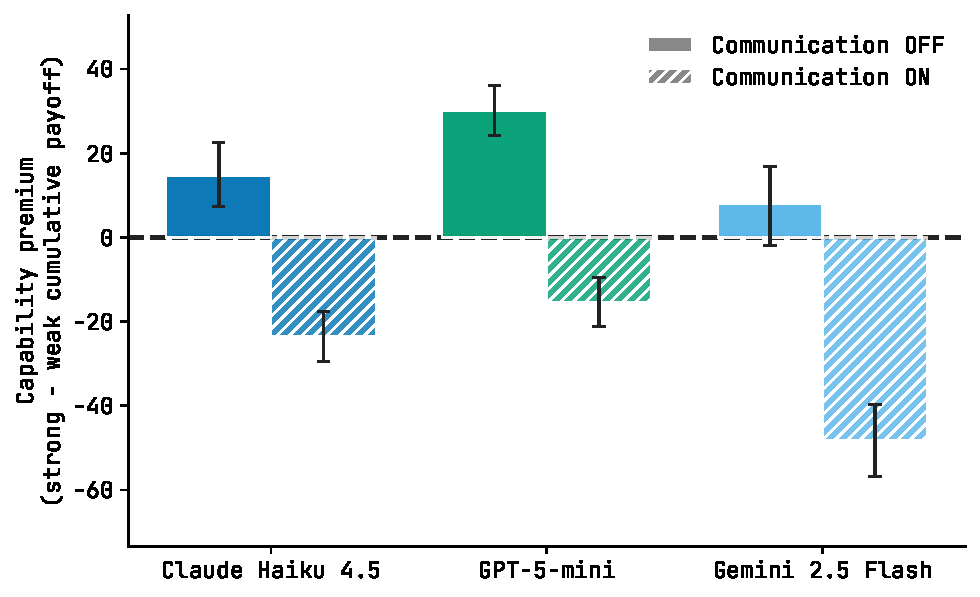
\includegraphics[width=0.85\textwidth]{f1_premium_by_communication.pdf}
\caption{The capability premium (strong minus weak cumulative payoff) for each strong
model against the weak Llama agents in the same mixed Public Goods games, with
communication off (solid) and on (hatched). Bars are means over games with 95\%
bootstrap confidence intervals. Every model crosses from a positive premium to a
negative one.}
\label{fig:premium}
\end{figure}

A mixed-effects regression of payoff on tier, communication, and game, fit over the
mixed-tier games with a per-game random intercept, locates where the flip lives. (The
pre-registered model also specified a per-agent intercept, Section~\ref{sec:prereg};
with one end-of-game payoff per agent that intercept is not identifiable, so the model
fit here keeps only the per-game term, a disclosed departure from the plan.) The
three-way strong $\times$ communication $\times$ game interaction is $-37.7$
($p = 0.0001$): the communication-driven swing in the strong premium is specific to the
Public Goods Game, not shared with Trust, where the same communication term does not
reach significance ($p = 0.18$). That cross-game split is taken up in
Section~\ref{sec:res-dissociation}.

This gives the two hypotheses each a verdict. \textbf{H2}, that the capability premium
can run negative, holds: under communication the premium is negative in every mixed
Public Goods cell, with intervals that exclude zero, and each strong model individually
earns less than the weak one. \textbf{H3}, that communication is the lever, holds in the
Public Goods Game: switching it on moves the premium by roughly fifty tokens, from about
$+24$ to about $-30$, and the interaction term ties that swing to this game
($p = 0.0001$).

What communication does \emph{not} do is let the agents talk to one another. As
Section~\ref{sec:communication} sets out, a message is produced and logged but never
delivered; the only thing the condition adds to a round is the request to make a public
pledge, on top of the past contributions both conditions already show. The transcript
bears this out. The strong agent's appeals track what the others \emph{did}, never what
they said: \emph{``it seems some of us are contributing less''} follows the falling
contributions it can see, and no agent in the game ever answers another's words, because
no agent ever receives them. The inversion is real, but its lever is the framing of
being asked to commit in public, not an exchange of cheap talk. What that framing does
to a capable agent, and why the weak agents are untouched by it, is the subject of the
discussion (Chapter~\ref{ch:discussion}).

\section{H5: A game-dependent dissociation}
\label{sec:res-dissociation}

The headline lived in the Public Goods Game. H5 asks whether it travels: do the same
effects hold in the Trust Game, or reverse between the two? Figure~\ref{fig:dissociation}
sets the capability premium for both games side by side, communication off and on.

\begin{figure}[tbp]
\centering
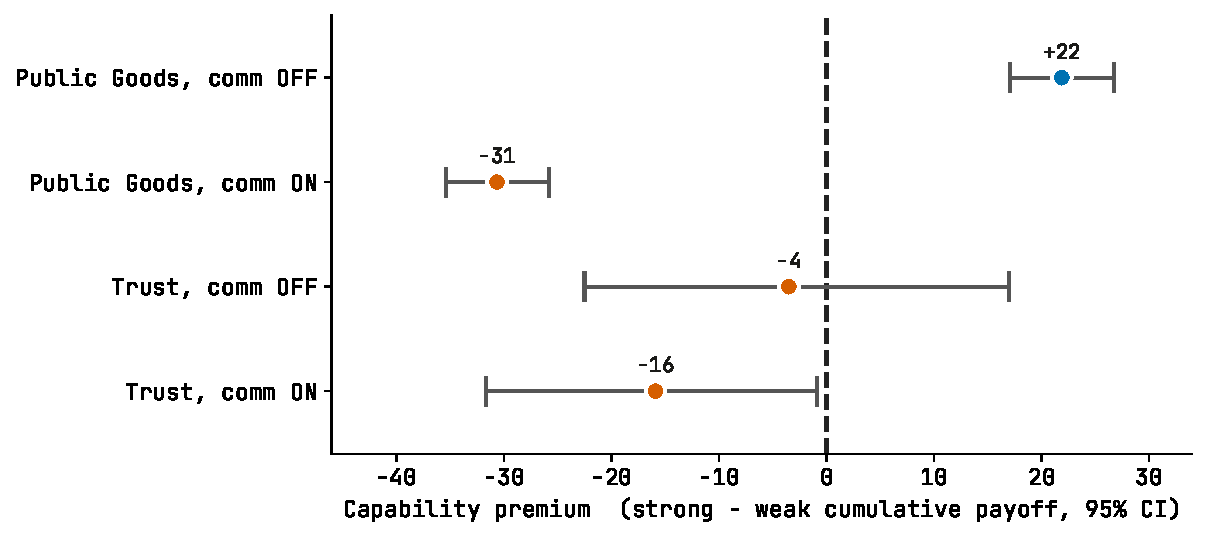
\includegraphics[width=0.82\textwidth]{f7_dissociation_by_game.pdf}
\caption{Capability premium (strong minus weak cumulative payoff) by game and
communication condition, point estimate with 95\% bootstrap confidence interval. The
Public Goods premium crosses from clearly positive to clearly negative; the Trust
premium stays near zero with intervals that barely separate from it.}
\label{fig:dissociation}
\end{figure}

The two games do not tell the same story. In the Public Goods Game the premium is
clearly positive without communication ($+21.9$, $[+17.1, +26.7]$) and clearly negative
with it ($-30.6$, $[-35.4, -25.8]$), the inversion of Section~\ref{sec:res-premium}. In
the Trust Game it sits near zero and stays uncertain: $-3.5$ ($[-22.5, +17.0]$) without
communication, $-15.9$ ($[-31.7, -0.9]$) with it. The off interval spans zero and the on
interval only just clears it.

H5's pre-registered falsification criterion is a sign reversal between the games: the
prediction would be refuted if the premium ran one way in one game and the opposite way
in the other. It does not. Under communication both premiums are negative, so H5 is not
falsified by its own test. But the predicted directional consistency is not confirmed
either. The Public Goods premium swings some fifty tokens across the communication
switch; the Trust premium barely moves and never separates cleanly from zero. The effect
keeps its sign where it can be measured, but its force belongs to the group game, not the
dyad.

This is a game-dependent dissociation, a sharper result than a flat failure to
replicate. Whatever communication does to a capable agent, it does in a four-player
public good, where one cooperator's contribution is visible to three others and
free-riding on it pays. The two-player Trust Game has no crowd to free-ride in, and there
the capability gap leaves almost no mark on payoffs. Why the group setting and not the
dyad is the question the discussion takes up (Chapter~\ref{ch:discussion}).

\section{H1: Welfare inequality (modest)}
\label{sec:res-inequality}

The substantive inequality in these games is the capability premium of
Section~\ref{sec:res-premium}, a tier-sized gap between who earns and who does not. The
welfare inequality H1 predicts, the spread of the payoff distribution as a whole, is
real but small, and small for a reason: most games are decided among agents who finish
close together, with the tier gap riding on top. Figure~\ref{fig:inequality} reads the
Gini coefficient of each game's final payoffs by composition.

\begin{figure}[tbp]
\centering
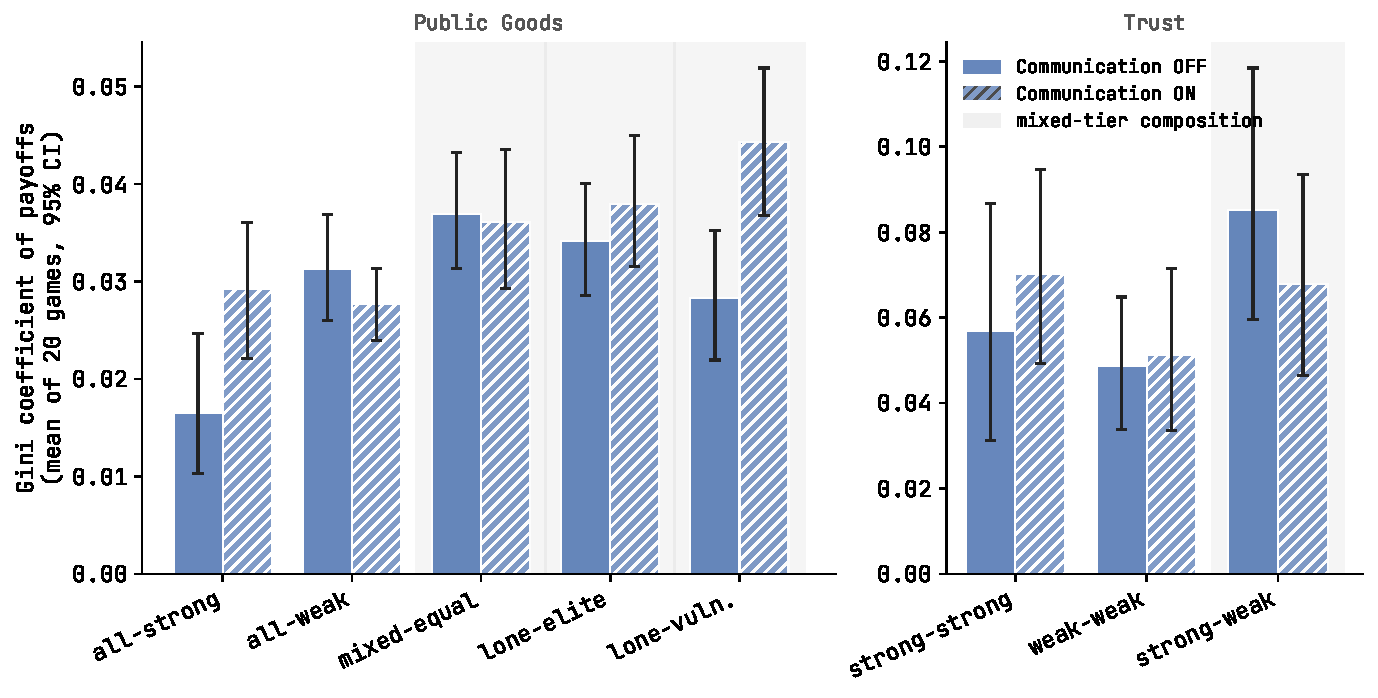
\includegraphics[width=\textwidth]{f2_inequality_by_composition.pdf}
\caption{Gini coefficient of final payoffs by composition and game, communication off
(solid) and on (hatched), mean over twenty games with 95\% bootstrap confidence
intervals. Mixed-tier compositions are shaded. Inequality is modestly higher in the
mixed and asymmetric populations.}
\label{fig:inequality}
\end{figure}

Two things hold at once. Mixed-tier populations are more unequal than homogeneous ones,
as predicted: in the Public Goods Game the mean Gini is $0.036$ across the mixed
compositions against $0.026$ across the homogeneous ones. And the gap is slight. A Gini
of $0.04$ describes a nearly flat distribution; with four players the index can climb to
$0.75$ before one agent holds the whole pie, so the inequality these games generate is a
faint version of what the coefficient can register.

The ordering survives the choice of index. The pre-registered Atkinson index, read at
all three inequality-aversion settings ($\varepsilon \in \{0.5, 1.0, 2.0\}$), agrees with
the Gini on the comparison that matters: mixed populations come out more unequal than
homogeneous ones at every setting. H1 holds in direction and stays small. Capability
asymmetry does widen the payoff distribution, but the welfare cost of that widening is
modest beside the tier-level redistribution the premium already described.

\section{H4: Deception, surprisal separates the tiers and policy-KL inverts}
\label{sec:res-deception}

Deception was pre-registered as exploratory, and it is the one finding two measures can
be made to agree on while a third, the control, runs the other way by design.
Figure~\ref{fig:deception} shows the two numeric signals over the 519 scored agent-games.

\begin{figure}[tbp]
\centering
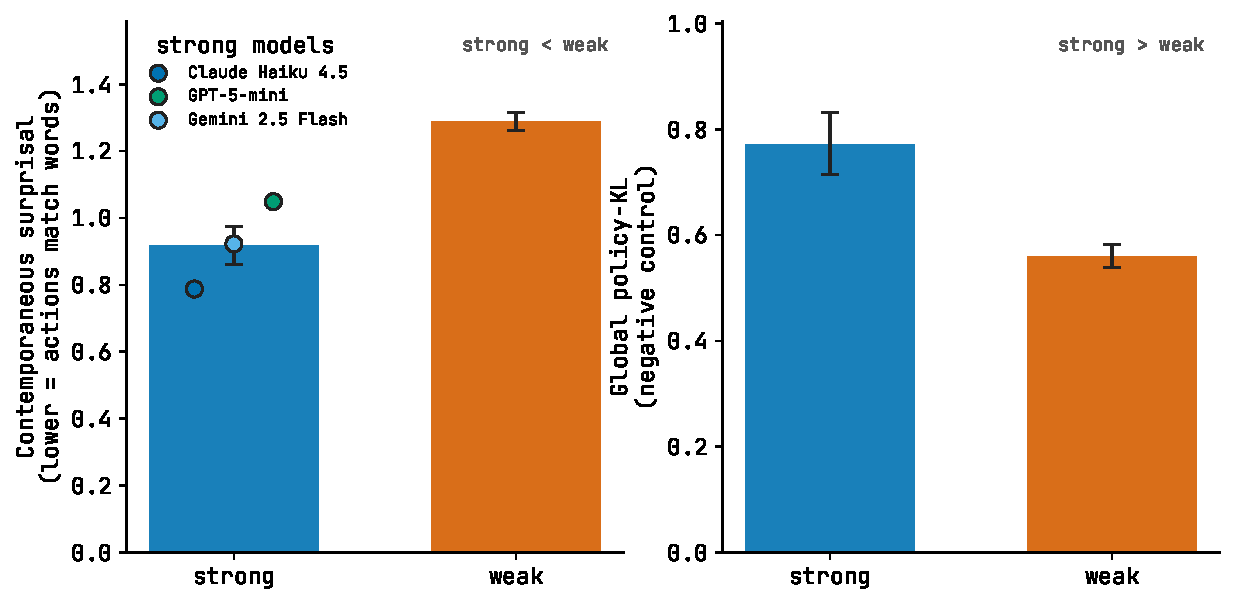
\includegraphics[width=0.92\textwidth]{f3_deception_surprisal_vs_kl.pdf}
\caption{Deception by tier over the scored agent-games. Left: contemporaneous surprisal
(lower means actions match words); the strong tier sits below the weak, and each strong
model below the weak mean. Right: the global policy-KL negative control, which runs the
opposite way. Bars are means with 95\% bootstrap confidence intervals.}
\label{fig:deception}
\end{figure}

By the contemporaneous surprisal, the validated signal, the weak tier is the deceptive
one. Surprisal, the negative log probability an agent's own stated policy gave to the
action it then took, averages $0.92$ ($[0.86, 0.97]$) for the strong tier and $1.29$
($[1.26, 1.32]$) for the weak, a separation of $-0.37$ ($[-0.43, -0.31]$) whose interval
clears zero. It holds across the strong models, each below the weak average: $0.79$ for
Claude Haiku~4.5, $0.92$ for Gemini~2.5 Flash, $1.05$ for GPT-5-mini. The weak agents'
actions land where their own words gave least weight; the strong agents mostly do what
they said they would.

The global policy-KL, kept as a negative control, points the other way: $0.77$ ($[0.72,
0.83]$) for the strong tier against $0.56$ ($[0.54, 0.58]$) for the weak, the strong
scoring as \emph{more} deceptive. This is the artefact Section~\ref{subsec:deception}
anticipated. Policy-KL rewards a concentrated action distribution, and the strong agents,
who cooperate steadily, hold the most concentrated distributions of all, so the measure
reads their consistency as divergence. That the control inverts exactly where the
surprisal separates is what marks the contemporaneous signal, and not any
stated-versus-revealed gap, as the one that tracks deception.

\begin{figure}[tbp]
\centering
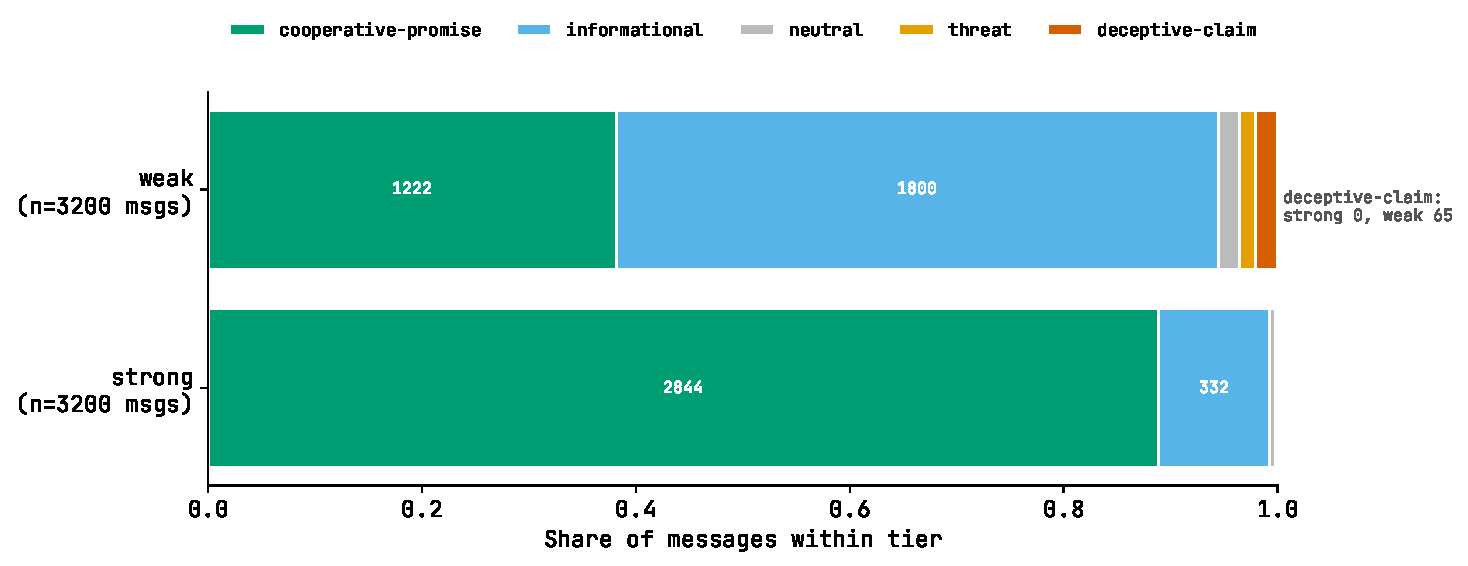
\includegraphics[width=0.95\textwidth]{f4_message_classes_by_tier.pdf}
\caption{Message classes by tier (communication on), assigned by a classifier that reads
the message and never the action. Of 3{,}200 messages per tier, the strong agents speak
almost entirely in cooperative promises; the weak tier carries the informational,
threat, and deceptive-claim mass.}
\label{fig:message-classes}
\end{figure}

The blind message classifier, which reads a message and never the action behind it,
reaches the same tier from the text alone. Of the 3,200 strong messages it labelled,
2,844 (89\%) are cooperative promises and not one is a deceptive claim; among the 3,200
weak messages the cooperative-promise share falls to 38\%, and the weak tier holds every
one of the 65 deceptive-claim labels and 49 of the 56 threats. So two independent
measures agree that the weak agents are the ones whose words and deeds diverge, a
behavioral surprisal validated against human labels and a text-only classifier blind to
behavior. The negative control running the other way is the point, not a contradiction:
it shows that the agreement between the first two is signal, not something any
stated-versus-revealed comparison would have produced.

\section{Behavioral tier inference (secondary outcome)}
\label{sec:res-tier}

Capability tier is not one of the five hypotheses; it is a secondary, descriptive
question the pre-registration asked beside them. Can an observer recover an agent's tier
from how it played, with no access to its name? A logistic regression on five behavioral
features of a Public Goods agent, the mean and the variance of its contribution, the
trend across rounds, the end-game drop, and a reciprocity term, answers yes, though not
perfectly. Figure~\ref{fig:tier} reports it under five-fold cross-validation.

\begin{figure}[tbp]
\centering
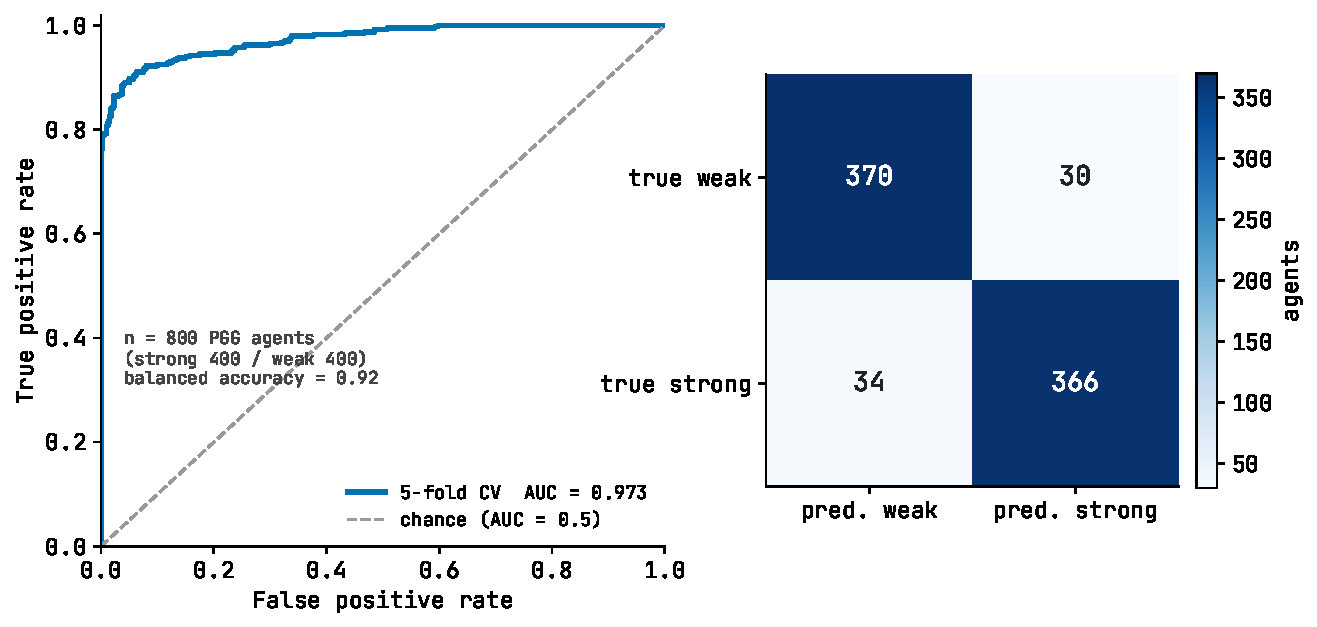
\includegraphics[width=0.92\textwidth]{f6_tier_inference_roc.pdf}
\caption{Tier inference from behavior on the 800 Public Goods agents, evenly split
between tiers. Left: the cross-validated ROC curve against the chance diagonal. Right:
the confusion matrix at a probability threshold of one half. The classifier separates
the tiers well but not perfectly.}
\label{fig:tier}
\end{figure}

Across the 800 Public Goods agents, four hundred to a tier, the classifier reaches an
area under the ROC curve of $0.973$ and a balanced accuracy of $0.92$ against a chance
baseline of $0.50$. The errors are near-symmetric: of four hundred strong agents it
labels 366 correctly, and of four hundred weak agents 370. The feature that carries the
most weight is the variance of contribution (coefficient $-3.49$): a steady hand marks
the strong tier and an erratic one the weak, the same consistency the premium and
deception results turned on, read here as a fingerprint.

A high score that is not a ceiling is the honest outcome rather than a disappointing
one. A perfect separator would mean the three strong models share a signature so rigid
that the classifier is naming the model, not the capability; the agents it misses are
the games where a strong agent played like a weak one or the reverse, the variation a
capability difference should still leave room for.

\section{Interaction networks (secondary)}
\label{sec:res-networks}

The last secondary outcome reads the games as networks rather than as payoff
distributions. Two graphs were built, and they differ in how much weight they can carry.

\begin{figure}[tbp]
\centering
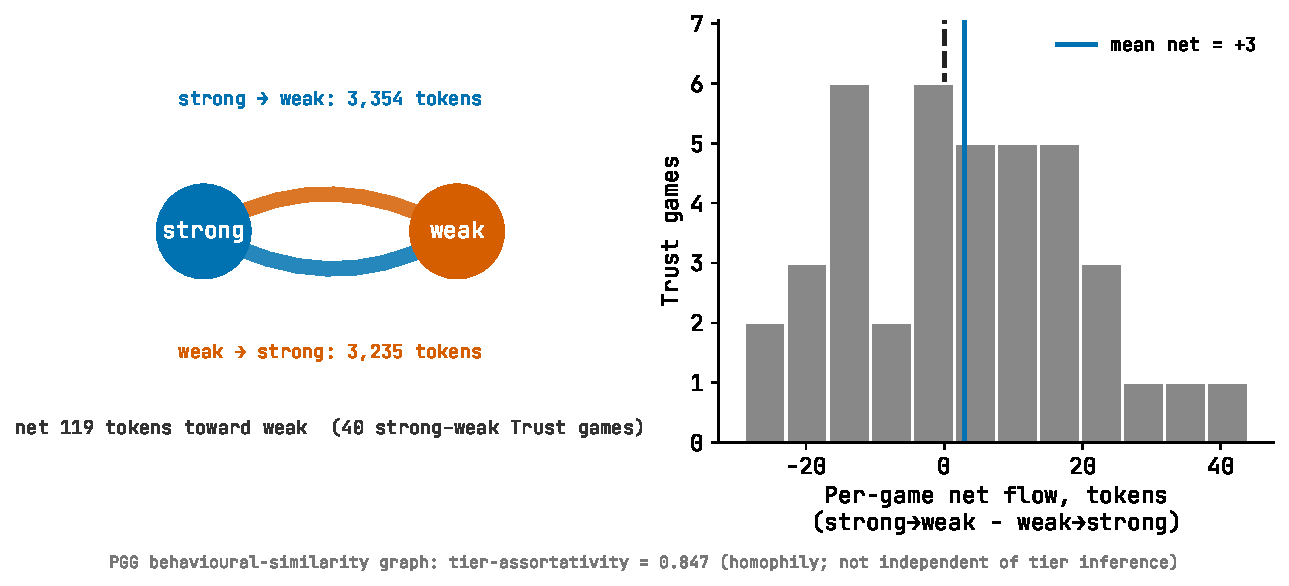
\includegraphics[width=\textwidth]{f5_trust_token_transfer.pdf}
\caption{Token flow in the forty strong-weak Trust games. Left: the aggregate
strong-to-weak and weak-to-strong totals, with the net. Right: the per-game net flow.
The tier-assortativity printed below belongs to a separate behavioral-similarity graph,
not this transfer graph, and is shown caveated.}
\label{fig:network}
\end{figure}

The first is a genuine interaction graph: in the strong-weak Trust games, who sent
tokens to whom. Across the forty such games the flow is nearly balanced, $3{,}354$
tokens from strong to weak against $3{,}235$ the other way, a net of $119$ toward the
weak. It is a small asymmetry in the same direction as the Trust premium, and as modest
as that premium was. The second graph is built not from transfers but from behavioral
similarity, linking agents that played alike. On it the strong tier is mildly more
central (eigenvector centrality $0.035$ against the weak tier's $0$), and same-tier
agents cluster, a tier-assortativity of $0.847$.

That second number wants reading with care, and the figure says so. The similarity graph
is built from the very features the tier classifier of Section~\ref{sec:res-tier} uses,
so its assortativity is not independent evidence of clustering; it largely restates, in
the language of a graph, that the tiers behave differently. The transfer graph is the one
that records an interaction the agents actually had.

\section{Findings against hypotheses}
\label{sec:res-summary}

Table~\ref{tab:findings} sets each registered prediction against what the data showed,
one row per hypothesis, so the pre-registration and the outcome read side by side. The
two findings that carry the thesis are H2 and H3, the negative premium and the
communication framing that produces it; H1, H4, and H5 place that result, and the two
secondary outcomes describe the agents it is about. Why the premium inverts, and why only
in the group game, is the work of the next chapter.

\begin{table}[h!]
\centering
\small
\caption{Each pre-registered prediction (osf.io/rnqgs) against the production outcome.
H2 and H3 carry separate verdicts though they share Section~\ref{sec:res-premium}.}
\label{tab:findings}
\begin{tabular}{@{}l p{5.2cm} p{8.4cm}@{}}
\toprule
 & Registered prediction & Outcome \\
\midrule
H1 & Mixed-tier populations are more unequal than homogeneous ones &
  Supported, modest. PGG Gini $0.036$ vs $0.026$; Atkinson agrees at every $\varepsilon$. \\
H2 & The strong tier need not out-earn the weak, and may earn less &
  Supported. Under communication the premium is negative in every mixed PGG cell. \\
H3 & Communication worsens the strong tier's premium &
  Supported in the Public Goods Game ($+24 \to -30$; interaction $p = 0.0001$); absent in Trust. \\
H4 & Surprisal tracks deception better than the global policy-KL &
  Supported, exploratory. Surprisal separates the tiers; policy-KL inverts as the negative control. \\
H5 & The effects hold across the two games without reversing &
  Not falsified (no sign reversal), but consistency not confirmed: a game-dependent dissociation. \\
\midrule
\multicolumn{3}{@{}l}{\textit{Secondary outcomes (descriptive, not hypotheses)}} \\
Tier & Tier is recoverable from behavior alone &
  ROC AUC $0.97$, balanced accuracy $0.92$ ($n = 800$ PGG agents). \\
Network & Interaction structure differs by tier &
  Net Trust flow $119$ tokens toward the weak; similarity clustering not independent of the row above. \\
\bottomrule
\end{tabular}
\end{table}

\chapter{Discussion}
\label{ch:discussion}

\section{Interpreting the inverted premium: commitment without reception}
\label{sec:disc-premium}

The headline result is a reversal: without communication the strong models out-earn the
weak, and with it they fall behind. The natural reading of that sentence is the wrong one.
``Communication'' suggests the weak agents heard the strong agents' cooperative promises and
took advantage of them, but that is not what the apparatus does. As
Section~\ref{sec:communication} sets out, a message is produced and logged and never
delivered; no agent in any game reads another's words. Whatever inverts the premium does so
without a single pledge changing hands.

What the communication condition actually adds to a round is one thing: the request that an
agent state a public intention before it acts. The behavior that follows says the request is
enough. Asked to commit, the capable models commit, and then they keep the commitment. The
transcript in Section~\ref{sec:res-premium} is typical: a strong agent announces it will give
its whole endowment and does so in every round, while the weak agents around it contribute a
fraction and pocket the rest. The strong agent is not exploited because anyone read its
promise; it is exploited because it cooperates, visibly, and the visible contribution is what
the others free-ride on. The history they all see carries contributions, and a steady high
contribution is a standing invitation to give less.

The asymmetry, then, is in who honors a stated intention. Both tiers are asked to pledge, and
both pledge cooperatively: the classifier of Section~\ref{sec:res-deception} labels nearly
nine in ten strong messages as cooperative promises. The difference is the follow-through. The
capable models act on the commitment they articulated; the weak models say the same words and
then do otherwise, which is exactly what their higher surprisal records. A public commitment
moves the one who makes it, and moves the capable more than the weak, because only the capable
treat their own stated policy as binding. That is why the effect needs no audience: the
commitment does its work on the committer.

This is a narrower and stranger claim than the word ``communication'' invites, and its size is
worth being exact about. The study does not show that talking helps weak agents exploit strong
ones, nor that cheap talk coordinates a group. It shows that asking a capable agent to say what
it will do makes it more likely to do the cooperative thing it said, at a cost, in a setting
where cooperation can be taken advantage of. This sits beside a recent result that runs the
other way. \emph{More Capable, Less Cooperative}~\cite{morecapable2026} finds that where helping
is free, more capable models can cooperate \emph{less}, withholding help they would lose nothing
by giving; here the capable models cooperate \emph{more}, and are punished for it. The two are not
in tension but two faces of one decoupling of capability from cooperative advantage, in one case
failing to produce cooperation that costs nothing, in the other producing cooperation that is
exploited. What this study adds is the lever, a public pledge, and the setting, a group dilemma,
in which the second face appears.

\section{Why the dissociation matters: group vs. dyadic structure}
\label{sec:disc-dissociation}

The inversion is a fact about the Public Goods Game. In the Trust Game the same populations
produce a premium that sits near zero and never separates cleanly from it
(Section~\ref{sec:res-dissociation}). Read carelessly, that looks like a failure to replicate;
read for what it is, it locates the effect. The two games differ in one structural way that
matters here, and the difference is why the lever pulls in one and not the other.

The Public Goods Game has a crowd. Four players draw on a shared pool, and one agent's
contribution is visible to, and divisible among, the other three. A capable agent that commits
to contributing creates exactly what free-riding needs: a standing benefit others can take a
share of without paying in. The commitment and the crowd are both required. Take away the
commitment and the strong agent contributes no more than anyone else; take away the crowd and
no one is positioned to free-ride on its contribution. The Trust Game removes the crowd. It is a
dyad, and its second mover faces a direct choice of how much to return, not a chance to draw
quietly from a pool someone else filled. A capable trustee can keep the tripled stake, but doing
so is a visible refusal to one partner, not an anonymous skim from a group.

The dissociation is the cross-game design earning its place. Had the study run only the Public
Goods Game, the inverted premium could have read as a general property of capable agents in
mixed company. Running the Trust Game beside it shows that it is not: the effect needs group
structure, a shared resource and an audience of beneficiaries, and fades where that structure is
absent. That is more useful than a uniform effect would have been, because it says where to
expect the behavior and where not to. The pre-registered test for H5 asked whether the effects
reverse between the games; they do not, so the prediction is not falsified by its own criterion
(Section~\ref{sec:res-dissociation}). The stronger reading is the dissociation itself: the
capability premium and its inversion are phenomena of the group game.

\section{A methodological contribution: a valid vs. an artefactual deception measure}
\label{sec:disc-deception}

The deception result is also a methodological one, because two measures built on the same idea
disagree, and the disagreement is the point. Both ask the stated-versus-revealed question a
forced-choice study put to single decisions~\cite{alignmentrevisited2025}: does an agent's
action match the policy its words implied? Lifted to a repeated game, the question splits into
two measures that need not agree, and here they point opposite ways.

The contemporaneous surprisal pairs each message with the action of the same round and asks how
much weight the stated policy gave to the move actually made. By it, the weak tier is the
deceptive one, and the blind classifier, which never sees an action, reaches the same verdict
from the text alone (Section~\ref{sec:res-deception}). The global policy-KL instead compares an
agent's whole-game distribution of actions against its stated policies, and it calls the strong
tier the deceptive one, which is backwards. The reason is concentration, not deceit. A steady
cooperator has a sharp action distribution, and a sharp distribution diverges far from any hedged
statement of intent, so the measure scores consistency as dishonesty: the most reliable agents
come out looking the least honest.

This is why the thesis keeps the global divergence only as a negative control and reports the
contemporaneous surprisal as the signal. The contribution is less a new metric than a
demonstration that the obvious one fails in a specific, instructive way. A stated-versus-revealed
gap measured over pooled behavior confounds deception with regularity; only the action-by-action
version, scored where a word meets the deed it was meant to predict, separates the two. A measure
that called the steadiest cooperators the worst liars would have quietly produced the wrong
story, and reporting it beside the one that works, rather than dropping it, is what lets the
deception finding rest on the agreement of methods rather than the luck of a choice.

\section{Implications for deploying mixed agent systems}
\label{sec:disc-implications}

If capable and weak language models are going to share tasks, and increasingly they will, the
result carries a few practical warnings. The first is that capability does not buy advantage in a
shared-resource setting. A stronger model dropped into a group that draws on a common pool can
end up subsidizing the others, and the asymmetry is largest exactly where the design might seem
safest, when the capable agent is asked to be transparent about what it means to do. Asking an
agent to declare its plan is a common move in alignment and oversight; in a group dilemma it is
the move that costs the capable agent most, because it turns a private disposition to cooperate
into a public, exploitable commitment.

The second warning is about measuring honesty in these systems. A deployer who wants to flag
deceptive agents has an obvious tool, the divergence between what an agent says and what it does,
and the obvious form of that tool is wrong in a way that matters: pooled over a run, it fingers
the most consistent cooperators and misses the agents whose words and deeds part company turn by
turn. The measure has to be contemporaneous to mean anything. The third is a scope condition more
than a warning: the effect is a property of group structure, not of capability as such, so a
one-on-one delegation between a strong and a weak model is a different situation from a many-agent
commons and should not be expected to behave the same way.

None of this is a deployment study, and the distance between four language models in a tokenized
game and a working multi-agent system is wide. What the results offer is not a prediction about
production but a caution about intuitions: that the strong agent will dominate, that letting
agents talk can only help, and that any reasonable measure of stated-versus-revealed behavior
captures deception. All three are natural, and all three are wrong in the settings studied here.

\section{Limitations}
\label{sec:disc-limitations}

The honest reading of these results depends on holding several limitations in view at once, most
recorded already where they arose and gathered here so none is lost.

The first concerns the communication condition, and it is the most important. What the study
calls communication is not an exchange. Each agent is asked to make a public pledge and is told
the others will see it, but the runner never delivers the message
(Section~\ref{sec:communication}); agents act on the contribution history, not on each other's
words. The condition is public commitment without reception, and every claim about it here is
meant in those terms. The word overstates the apparatus, and the finding is the narrower one of
Section~\ref{sec:disc-premium}, not a result about agents reading and answering one another.

The deception measures carry their own caveats, declared with the metric. The model that scores
an agent's stated policy is Claude Haiku~4.5, which also plays as one of the strong agents, so
the scorer is in part one of the scored (Section~\ref{sec:integrity}); the coupling is mitigated
by reading the same conclusion off three methods that share no machinery, the contemporaneous
surprisal, a blind text classifier, and the global divergence that runs the other way as a
control, rather than off any single read. The surprisal was validated against human labels by a
single rater, the metric's author, working blind and single-pass against a fixed rubric, and it
cleared significance but not the pre-registered correlation bar, which is why it is reported as
exploratory rather than confirmatory. These are real limits on how much the deception result can
bear; it is offered as a methodological demonstration and a convergence of signals, not a
calibrated measurement.

The capability axis is coarse. ``Strong'' means three specific frontier models and ``weak'' means
one small local one, and the tiers differ in more than a single dimension of capability, so the
results speak to that contrast rather than to capability as a clean variable. The scale is modest
too: 320 games, with the per-game deception divergence sparse enough that the signal lives in the
spread across games rather than in any one of them. The primary regression keeps only a per-game
random intercept where the pre-registration named one for agents as well, because the modelled
outcome is a single end-of-game payoff per agent (Section~\ref{sec:res-premium}); the models'
outputs are not bit-reproducible regardless of seed; and the network reading of
Section~\ref{sec:res-networks} draws on the same behavioral features as the tier classifier, so
the two are not independent evidence. None of these sinks the central results, which are large
and consistent, but each marks a place where the reader should not ask the data for more than it
holds.

\section{Future work}
\label{sec:disc-future}

The clearest next step follows from the mechanism. If a public commitment changes behavior
without being received, the experiment to run is to vary reception directly: deliver the messages
in one condition and withhold them in another, holding the pledge-request fixed, and see whether
being read changes what a commitment does. The present design cannot separate the request to
pledge from the claim that others will see it, because it never delivers; a channel that actually
carried messages would let the framing effect and any genuine exchange effect be told apart, and
would test whether the inversion survives once the audience is real.

Two other extensions would firm up what the results can claim. The capability axis wants
widening, from three strong models against one weak to a graded set that varies capability while
holding other differences as nearly fixed as possible, so that ``capability'' becomes something
closer to a measured variable than a contrast between a frontier API and a small local model. And
the deception measure wants the validation the pilot only sketched: more messages, more than one
rater, and a labeling effort large enough to say whether the contemporaneous surprisal tracks
human judgments well enough to stand on its own rather than only in the company of other signals.
Beyond these, the dissociation invites a map. Varying group size and the structure of the shared
resource would trace the boundary that the Public Goods and Trust games mark at only two points,
and show how much of a crowd a commitment needs before it can be exploited.

\chapter{Conclusion}
\label{ch:conclusion}

This thesis asked what happens when language models of different capability share an economy, and
returned an answer that inverts the obvious one. The capable models do not reliably dominate the
weak. With no channel between them the strong earn a premium; but when each agent is asked to make
a public pledge before it acts, the premium turns negative and the strong earn less. The pledge is
never delivered to anyone. What changes behavior is the act of committing in public, and only the
capable models treat their own stated intention as binding: they cooperate on it, contribute
visibly, and are free-ridden by the others through the shared pool. The effect belongs to the group
game and fades in the two-player exchange, which places it in the structure of the commons rather
than in capability itself.

The second finding is a measure rather than a phenomenon. Asked whether the agents deceive, the
obvious divergence between stated and revealed policy gives the wrong answer, calling the steadiest
cooperators the least honest; a contemporaneous, action-by-action surprisal gives the right one. The
contribution is in reporting the two together, the signal and the artefact that mimics it, rather
than quietly keeping the measure that flatters the story. Both results were fixed in direction
before the first game ran, which is the strongest thing the thesis can say for them: they are not
what it set out to find. For anyone assembling systems out of agents of unequal capability, that is
the warning worth keeping: the strong do not simply win, and the familiar ways of managing them,
asking them to be transparent and checking whether they lie, can misfire unless the structure they
act in and the measure used on them are chosen with care.


% ================= BIBLIOGRAPHY =================
\addcontentsline{toc}{chapter}{References}
\bibliographystyle{IEEEtran}
\bibliography{references}

\end{document}
